% !TeX root = draft_ftsfr.tex
\documentclass{article}

% Language setting
% Replace `english' with e.g. `spanish' to change the document language
\usepackage[english]{babel}

% Set page size and margins
% Replace `letterpaper' with`a4paper' for UK/EU standard size
\usepackage[letterpaper,top=2cm,bottom=2cm,left=3cm,right=3cm,marginparwidth=1.75cm]{geometry}

% Useful packages
\usepackage{amsmath}
\usepackage{graphicx}
\usepackage[colorlinks=true, allcolors=blue]{hyperref}
\usepackage{natbib}  % Required for JPE bibliography style
\usepackage{booktabs} % For better tables
\usepackage{multirow} % For tables with merged cells
\usepackage{hyperref} % For links
\usepackage{setspace}
\usepackage{placeins}
\usepackage{subfig} % For subfigures (modern replacement for subfigure)
\usepackage[page]{appendix}

\usepackage{float} % For forcing figure placement with [H]
\usepackage[table]{xcolor} % For coloring table cells

% \title{An Open-Source Financial Time Series Forecasting Benchmark}
\title{Benchmarking Forecasting Methods for Financial Stability}
\author{
        Jeremiah Bejarano\thanks{Office of Financial Research, U.S. Department of the Treasury and the Financial Mathematics program at the University of Chicago} \footnote{All mistakes are my own. Views and opinions expressed are those of the authors and do not necessarily represent official positions or policy of the Office of Financial Research (OFR) or the U.S. Department of the Treasury. Please address correspondence to \href{mailto:jeremiah.bejarano@ofr.treasury.gov}{jeremiah.bejarano@ofr.treasury.gov}.} 
        \and
        Viren Desai\footnotemark[3]
        \and 
        Kausthub Keshava\footnotemark[3]
        \and
        Arsh Kumar\footnotemark[3]
        \and
        Zixiao Wang\thanks{Most of this work was completed as a student in the Financial Mathematics program at the University of Chicago}
        \and
        Vincent Hanyang Xu\footnotemark[3]
    }
\date{\today}

\begin{document}
\maketitle

% \begin{abstract}
% This paper presents an open-source finance data repository for
% benchmarking the performance of global time series forecasting methods and
% compares the performance of many of the most popular modern methods. A
% standardized benchmark is crucial for comparing the performance of different
% forecasting methods, so as to allow apples-to-apples comparisons across
% different forecasting methods and to discourage cherry-picking of results.
% Despite the ubiquity of time series forecasting methods in macroeconomics and
% finance, a standardized repository of data for benchmarking in these domains
% does not exist. One reason for this is that many of these datasets are available
% only through paid subscriptions and are thus not freely distributable. To
% address this issue, we instead provide a set of scripts that automate the
% download, data cleaning, and assembly of data sets from the Wharton Research
% Data Services (WRDS) platform and the Bloomberg Terminal. Since many academic
% institutions have access to WRDS or a Bloomberg Terminal, contingent on having
% access to the appropriate WRDS or Bloomberg subscriptions, each researcher will
% be able to exactly reproduce each of the datasets provided in this repository.
% Furthermore, the datasets that we provide are cleaned and formatted in a way
% that matches best practices established within the corresponding academic
% literature. Our aim is to facilitate the process of benchmarking global times
% series forecasting methods on data from these domains. In this light, we
% demonstrate the utility of our repository by benchmarking the performance of a
% suite of classical and modern forecasting methods. We hope that this repository
% will enhance research that increases the precision of financial and economic
% forecasts and contribute to research related to promoting financial stability
% and supporting a well-functioning economy.
% \end{abstract}


\begin{abstract}
    Financial regulators and researchers increasingly emphasize forward-looking risk monitoring to preemptively address systemic vulnerabilities. This paper benchmarks state-of-the-art global time series forecasting methods, which have proven superior in the time series literature, on a comprehensive suite of financial stability indicators. Benchmarks drive progress, and our systematic evaluation of 24 forecasting methods ranging from classical models to modern deep learning architectures reveals which approaches best capture early warning signals across different market segments. We evaluate these methods on critical financial stability metrics including arbitrage basis spreads that signal funding market stress, banking indicators that reveal institutional vulnerabilities, and asset returns across multiple markets. To enable reproducible research and continuous improvement in financial forecasting, we develop an open-source \emph{financial time series forecasting repository} that standardizes these datasets according to canonical academic methodologies. Our results provide financial stability authorities with evidence-based guidance on which forecasting approaches most reliably detect emerging risks in specific market segments, directly enhancing the toolkit for macroprudential surveillance and systemic risk monitoring.
    \end{abstract}

\section{Introduction}
\label{sec:introduction}
\doublespacing

% TODO: Write introduction emphasizing the critical need for standardized benchmarks in finance
% - Establish that time series forecasting is ubiquitous and prevalent in macroeconomics and finance domains
% - Highlight the current gap: no existing standardized benchmarks for evaluating forecasting algorithms in macro-finance
% - Explain why apples-to-apples comparisons are impossible without standardized datasets
% - Stress that researchers currently evaluate their own models on arbitrarily chosen datasets, making comparisons meaningless
% - Position this work as filling a critical gap in quantitative finance research
% - Emphasize that this complements (not substitutes) the Monash benchmark
% - Make clear that the lack of standardization is particularly problematic in finance where data often requires subscriptions

% Why forecasting is important for financial stability
Financial regulators and researchers increasingly emphasize forward-looking risk monitoring to preemptively address systemic vulnerabilities\footnote{
    See the following examples. The Office of Financial Research's (OFR) Annual Report of 2022 states ``The OFR has and will continue to monitor and analyze risks to financial
    stability, remaining agile to identify and examine emerging threats as they arise now and in the coming years." 
    According to the Financial Stability Oversight Council's (FSOC) 2024 Annual Report, ``The Systemic Risk Committee `supports the Council's efforts in identifying risks and responding to emerging threats
    ... and has been using the Analytic Framework to identify and evaluate vulnerabilities and build consensus regarding risk priorities.' " (See \url{https://home.treasury.gov/system/files/261/FSOC2024AnnualReport.pdf}.)
    According to their the Federal Reserve's Financial Stability documentation, ``The Federal Reserve maintains a flexible, forward-looking financial stability monitoring program to help inform policymakers of the financial system's vulnerabilities to a range of potential adverse events or shocks." (See \url{https://www.federalreserve.gov/financial-stability/proactive-monitoring-of-markets-and-institutions.htm}.) 
    As another example, the Large Institution Supervision Coordinating Committee (LISCC) was established ``based on lessons learned from the 2007-09 global financial crisis that revealed deficiencies in how large, systemically important firms had been supervised. These lessons underscored the need for the supervision of the largest firms to be more forward-looking, consistent, and informed by analysis from multiple perspectives and disciplines". (See \url{https://www.federalreserve.gov/supervisionreg/large-institution-supervision.htm}.)
} \citep{Adrian2015}. 
In this context, improving our ability to forecast key financial metrics is not a theoretical exercise. Rather,
it is critical for early warning signals and timely policy responses. 
% The Office of Financial Research (OFR) and the Financial Stability Oversight Council (FSOC) were established to identify emerging risks across financial markets. However, their effectiveness hinges on robust data and predictive analytics. 
By developing an open-source financial time series forecasting benchmark, we directly enhance the toolkit available for financial stability monitoring. This benchmark brings together a wide range of datasets---spanning asset returns, arbitrage (basis) spreads, and banking indicators---that are crucial for assessing vulnerabilities in different corners of the financial system. Importantly, it evaluates state-of-the-art ``global" forecasting methods (which learn across many time series) and compares them to classical models, shedding light on which approaches best capture early signs of stress in these data. In sum, better forecasting of these metrics can help regulators and market participants spot trouble on the horizon, informing pre-emptive measures to safeguard the economy

% Why we need a standardized benchmark
The time-series forecasting community increasingly recognizes the need for standardized evaluation frameworks. 
Benchmarks drive progress.
Until recently, the absence of standardized benchmark datasets meant that most studies evaluated their methods on limited, arbitrarily selected time series or domain-specific data, making meaningful comparisons across methods virtually impossible. As \citet{Prater2024} note, this lack of standardization has resulted in ``poor quality evaluations" and irreproducible comparisons across forecasting studies. While several benchmark repositories have emerged to address this gap, they remain limited in their coverage of financial markets. 
The FRED-MD database \citep{McCracken2016} provides a valuable collection of 134 U.S. macroeconomic series, but focuses primarily on real economic indicators rather than financial market data. The FinTSB benchmark \citep{Hu2018} includes equity returns, though it may not leverage CRSP, widely regarded as the gold standard for high-quality equity market data. Meanwhile, the UCR Time Series Classification Archive \citep{Dau2019} and UEA Multivariate Time Series Classification Archive \citep{Bagnall2018} and MUU Extrinsic Regression Repository \citep{Tan2020} do not include coverage of the financial domain.
The Monash repository \citep{Godahewa2021} and recent efforts like TFB \citep{Qiu2024} have made strides toward broader coverage, yet comprehensive representation of financial asset classes, from corporate bonds to credit derivatives, remains absent. (See Table \ref{tab:benchmarks} for a summary of existing benchmarks.) This gap is particularly problematic given that, according to the ``No Free Lunch" Theorem \citep{Wolpert1997},
there is no single forecasting method that performs best for all time series. As such, to improve forecasting in the financial domain, we need to evaluate forecasting methods on a suite of datasets from the financial domain and, importantly,
these datasets need to reflect the form of the data as they commonly appear in the relevant finance literature. That is, they should use the same data sources and the same domain-specific cleaning and normalization procedures established in the literature. 


Our proposed benchmark addresses this limitation by creating a standardized, literature-compliant repository specifically designed for the finance domain. By providing open-source scripts that automate the download and cleaning of data from institutional sources like WRDS and Bloomberg, we enable researchers to reproduce exact datasets used in canonical finance papers. Our aim is to fill a critical gap in quantitative finance research by providing the first comprehensive forecasting benchmark tailored to financial markets. In particular, our paper has the following main contributions:

\begin{itemize}
    \item We introduce the first comprehensive time series forecasting archive focused specifically on financial markets, available at \url{https://jeremybejarano.com/ftsfr/}. This archive provides standardized datasets across multiple asset classes and market segments:
    \begin{itemize}
        \item Asset return series spanning equities, corporate bonds, U.S. Treasuries, sovereign bonds, foreign exchange rates, commodity futures, credit default swaps (CDS), and options
        \item Arbitrage basis spreads including covered interest parity (CIP) deviations, CDS-bond basis, Treasury-swap spreads, TIPS-Treasury spreads, equity spot-futures basis, Treasury spot-futures basis, and box spread arbitrage
        \item Specialized datasets critical for financial stability monitoring, including bank Call Report data, Treasury auction statistics, and yield curve dynamics
    \end{itemize}
    
    \item We provide validated implementations of canonical data cleaning procedures from seminal finance papers, each following the exact methodology of the original studies. Crucially, while these foundational papers often lack publicly available replication code, our implementations successfully reproduce their key results, establishing both the correctness of our data processing and creating a reusable framework for future research.
    
    \item We emphasize domain-specific data curation, recognizing that financial data requires specialized treatment reflecting market microstructure, regulatory requirements, and established academic conventions. Each dataset is processed using the precise subsample definitions, filters, and transformations specified in the corresponding literature, ensuring that forecasting evaluations reflect the actual data as used by domain experts rather than generic time series.
    
    \item We present comprehensive baseline forecasting results across all datasets using a suite of 24 methods ranging from classical statistical models (ARIMA, ETS, Theta) to modern machine learning approaches (CatBoost, neural networks) and state-of-the-art deep learning architectures (Transformer variants, N-BEATS, TimesFM). These baseline results enable standardized performance comparisons and establish benchmarks for future research.
    
    \item We provide novel insights into market-specific predictability by systematically evaluating forecasting performance across different asset classes and market segments. This analysis contributes to our understanding of where predictability exists in financial markets and can inform both academic research and policy decisions related to financial stability monitoring.
    
    \item All implementations are fully open source on \href{https://github.com/jmbejara/ftsfr}{GitHub} with best practices for reproducibility, including an automated data pipeline that pulls data from the appropriate data sources and cleans it according to the canonical methods established in the literature, and virtual environments ensuring perfect reproducibility across different computing environments.
\end{itemize}

By providing this resource, we enable the kind of standardized, apples-to-apples comparisons that have been lacking in financial forecasting research, while also contributing replication code for key papers and insights into predictability across financial markets.

\begin{table}[htbp]
\centering
% \footnotesize  % or 
\small
\caption{Existing Time Series Forecasting Benchmark Data Repositories}
\label{tab:benchmarks}
\begin{tabular}{llll}
\toprule
Source & Name & Coverage of Finance Domain & Website \\ 
\midrule
\cite{McCracken2016} & FRED-MD & US Macroeconomic Series & \href{https://www.stlouisfed.org/research/economists/mccracken/fred-databases}{Link}\\
\cite{Hu2018} & FinTSB & Equities Returns only & \href{https://github.com/TongjiFinLab/FinTSB}{Link}\\
\cite {Dau2019} & \begin{tabular}[t]{@{}l@{}}UCR Time Series\\Classification Archive\end{tabular}  & None & \href{https://www.cs.ucr.edu/%7Eeamonn/time_series_data_2018/}{Link}\\
\cite{Bagnall2018} & \begin{tabular}[t]{@{}l@{}}UEA Multivariate Time Series\\Classification Archive\end{tabular}  & None & \href{https://www.timeseriesclassification.com/}{Link}\\
\cite{Tan2020} & \begin{tabular}[t]{@{}l@{}}Monash, UEA \& UCR Time Series\\ Extrinsic Regression Repository\end{tabular} & None & \href{http://tseregression.org/}{Link}\\
\cite{Godahewa2021} & \begin{tabular}[t]{@{}l@{}}Monash Time Series\\Forecasting Repository\end{tabular} & Fred-MD is one component & \href{https://forecastingdata.org/}{Link}\\
\cite{Bauer2021} & Libra & Anonymous data, unclear & \href{https://github.com/DescartesResearch/ForecastBenchmark}{Link}\\
\cite{Qiu2024} & TFB & \begin{tabular}[t]{@{}l@{}}NN5 Bank Cash Withdrawals, \\Equity (NYSE/NASDAQ), \\ Foreign Exchange Rates \end{tabular} & \href{https://github.com/decisionintelligence/TFB}{Link}\\
\cite{Aksu2024} & GIFT-EVAL & Anonymous data, unclear & \href{https://github.com/SalesforceAIResearch/gift-eval}{Link}\\
\bottomrule
\end{tabular}
\end{table}


\section{Literature Review and Related Work}
\label{sec:literature}

% TODO: Position the paper relative to existing benchmarks and establish the canonical nature of chosen cleaning methods
% - Review the Monash Time Series Forecasting Archive and explain how FTSFR follows their established template
% - Introduce He, Kelly, Manela (2017) as the anchor paper for asset class selection and cleaning methods
% - Introduce Siriwardane, Sunderam, & Wallen (2022) "Segmented Arbitrage" as the anchor for arbitrage spread construction
% - Emphasize that the choice to follow these papers is deliberate - not doing anything novel is a FEATURE, not a bug
% - Acknowledge that some dataset choices are somewhat ad hoc but are anchored by these survey-style papers

\subsection{The Importance Of Open Source And Replicability}

Finance faces an active debate about a potential ``replication crisis.'' \cite{Jensen2023} find that predictors' average strength is only 54\% of the original strength outside the original sample, with 32\% becoming insignificant. While much of the debate centers around data snooping, some of it involves
coding and similar such bugs. There have been several high profile retractions\footnote{See  \cite{Lee2023} at \href{https://www.bloomberg.com/news/articles/2023-12-01/a-grad-school-number-cruncher-shakes-up-the-world-of-bond-quants}{Bloomberg}, and \cite{Dickerson2024}.}.
Despite disagreement on the crisis's extent, consensus exists at least on one way to help the situation: standardized, open source data infrastructure. \cite{Chen2022} demonstrate with their ``Open Source Cross-Sectional Asset Pricing'' project that transparent data construction, version control, and community validation can eliminate arbitrary researcher degrees of freedom. Such infrastructure prevents simple errors from invalidating years of research. For policymakers and financial regulators, standardized open source data 
helps them more effectively monitor systemic financial risks.

\subsection{Global Time Series Forecasting Methods}

The M-competition series is one of the most popular time series forecasting competitions in the field \citep{Makridakis1982, Makridakis2000, Makridakis2018, Makridakis2022}. Notably, the winning approaches of recent M-competitions have consisted of global forecasting models that train a single model across all series in the dataset. As \citet{Godahewa2021} observe, this pattern extends beyond the M-competitions. Winners of other major competitions including the NN3 and NN5 Neural Network competitions and various Kaggle competitions have similarly employed global models.

Global forecasting models represent a paradigm shift from traditional univariate approaches. Rather than fitting separate models to individual series, global models treat each series as a related instance within a larger dataset, extracting information from both temporal patterns within series and cross-sectional structure across the panel. This enables them to learn common patterns while accounting for series-specific variations, with particular advantages when forecasting related series—a common scenario in finance. Global methods can handle short series by borrowing strength from longer ones and provide robust parameter estimation through regularization. Recent implementations range from pooled regression to sophisticated deep learning architectures, with many demonstrating superior performance over traditional methods \citep{Godahewa2021}.

This paper contributes to the global forecasting literature by providing a comprehensive benchmark specifically designed for financial markets.
Our benchmark thus serves to improve the infrastructure for developing the next generation of forecasting methods tailored to the complexities of financial markets, potentially improving risk management, asset allocation, and financial stability monitoring.



\section{Datasets Included in the Benchmark}

In this section, we describe the datasets included in the benchmark. The datasets are organized into three main groups: asset class datasets, basis spread datasets, and other financial data. We provide brief description of each dataset below. Each datasets is constructed based off of a cleaning procedure from a well-known paper in the academic literature. To validate our cleaning and transformations, we replicate a key plot or table from each paper. We give brief details of this process below. Full details of the cleaning and replications are provided in the appendix.

% Please create a paragraph for each asset class and then within each paragraph, I don't want to talk about how the portfolios are constructed, but rather I want to talk about the essential cleaning, filtering, and transformations applied, because I want to stress to the reader why, like what is unique or interesting or what is our contribution by open sourcing the cleaning procedure used in this paper. So I guess for each, if you want to establish why is this paper considered canonical, And what are the essential filters and transformations applied by this paper? 

% A full detailed accounting of the cleaning procedure will be given later. These are short introduction glimpses of the why for each Each paragraph should be 2-3 sentences.

\subsection{Asset Class Datasets}
Our repository provides comprehensive datasets across seven major asset classes, each cleaned according to canonical methods established in the academic literature. We replicate each of the asset classes examined in \cite{He2017}, which are equities, US government and corporate bonds, foreign sovereign bonds, options, credit default swaps (CDS), commodities, and foreign exchange markets. 
This paper references a canonical paper in each asset class and uses the data cleaning procedures from that paper to construct test portfolios within that asset class.
For each asset class, we provide both aggregated portfolio returns (matching the test portfolios used in \cite{He2017}) and disaggregated security-level data. The disaggregated datasets apply identical filtering criteria, subsampling, and transformations as specified in the original papers, but preserve individual security information rather than aggregating into portfolios. 
To validate our data cleaning procedures, we replicate key summary statistics and cross-sectional patterns from each source paper cited within \cite{He2017}. For instance, our corporate bond portfolios match the credit spread patterns in \cite{Nozawa2017} and our options portfolios reproduce the volatility risk premium patterns found in \cite{Constantinides2013}. These validation exercises ensure that our standardized datasets faithfully represent the canonical cleaning methods established in the literature while providing a unified framework for cross-asset forecasting research. This approach allows researchers to both replicate existing studies (which typically use the aggregated portfolios) as well as to use the disaggregated data for richer analysis using the global time
series forecasting methods.



\paragraph{Equities}
For equities we adopt the canonical \cite{Fama1993} cleaning procedures. At a high level, this exclude ADRs, REITs, and firms with negative book equity, lag book-equity data by one fiscal year. We use data from the Center for Research in Security Prices (CRSP) and Compustat by Standard \& Poor's. These data sets
are the gold standard for research in equity markets. Altogether, this data and filtering procedures remove survivorship and look-ahead bias, and utilize the data as it's commonly used in asset pricing research for equities.


\paragraph{Treasuries} Our US Treasury bond portfolios utilize the CRSP Treasury database and follow \cite{Gurkaynak2007} procedure that underpins one of the
various yield curve data publications available on the Federal Reserve Board's website\footnote{See \url{https://www.federalreserve.gov/data/yield-curve-models.htm}}. At a high level, we keep only non-callable notes and bonds, strip out STRIPS/TIPS and other exotic issues, correct returns for accrued interest, and use strictly month-end transaction quotes. These filters remove optionality, stale prices, and auction-cycle noise that otherwise create spurious risk-premia. Open-sourcing the exact code lets anyone replicate this Treasury sample instead of relying on opaque heuristics.


\paragraph{Corporate Bonds}
We obtain corporate bond returns from the Open Source Bond Asset Pricing (OSBAP) project\footnote{See \url{https://openbondassetpricing.com/}}, which begins with the full TRACE transaction tape and then applies the market--microstructure--noise (MMN) correction procedure of \citet{Dickerson2024}.  Using MMN--adjusted ``clean'' prices is essential: the bid--ask--averaged quotes in raw TRACE embed a mechanical reversal that can be mis-interpreted as illiquidity and lead researchers to overstate corporate bond excess returns.  With the cleaned data we replicate and extend the ten value-weighted credit-spread deciles of \citet{Nozawa2017}, sorting on option-adjusted spreads each month.  Relative to unadjusted TRACE figures, the MMN correction eliminates roughly half of the apparent return spread and aligns liquidity estimates with quote-based ICE data, illustrating that much of the perceived illiquidity premium is an artefact of noise rather than compensation for trading frictions.  OSBAP also furnishes auxiliary fields such as modified duration, amount outstanding, coupon rate, and matched-Treasury yields, which we exploit later for duration-matched excess-return calculations. We validate our cleaning procedure by matching the construction of corporate bond portfolios in \cite{He2017}.

% \paragraph{Foreign Sovereign Bonds}
% For sovereign bonds, we implement the methodology of \cite{Borri2011}, creating 
% six portfolios based on a two-way sort using covariance with US equity returns and 
% S\&P credit ratings.


\paragraph{Options} The volume of SPX options traded has grown dramatically over time (along with the options asset class as a whole). Our monthly SPX options portfolio returns series follows the data cleaning and portfolio construction methodology of \citet{Constantinides2013} (``CJS'') which has become the canonical approach for constructing option-based portfolios. This framework forms the foundation for numerous studies in derivatives pricing and risk management. We then transform these portfolios into the option portfolios utilized in \citet{He2017} (``HKM''), in accordance with the procedure outlined in their paper. 

\begin{figure}[H]
  \centering
  \begin{tabular}{@{}c@{}}
    
\includegraphics[height=300pt,width=400pt]{../docs_src/spx_options_over_time.png}
  \end{tabular}
  \caption{The SPX options market has grown dramatically over time, particularly since the Global Financial Crisis.}
  \label{fig:spx_options_over_time}
\end{figure}


The \citet{Constantinides2013} portfolios are organized by option type (call or put), moneyness (9 levels), and maturity (3 levels), leading to $2 \times 9 \times 3 = 54$ distinct portfolios. The 18 portfolios in \citet{He2017} were constructed by taking an equal weight average across the 3 maturities for CJS portfolios with the same moneyness, adding $2 \times 9 = 18$ distinct portfolios to the dataset, for a total of 72 distinct SPX option portfolios. \emph{We have provided a simple coding system to identify individual portfolios and access these returns series.}

Our dataset is comprised of monthly leverage-adjusted portfolio returns for \textbf{all 72 SPX option portfolios, spanning 23 years from January 1996 to December 2019}. The 72 portfolio returns series were constructed from a raw daily dataset of approximately 19 million individual SPX option contracts. These portfolios are constructed using leverage-adjustments and daily dynamic rebalancing to maintain constant risk exposures over time.


The leverage adjustments and dynamic portfolio rebalancing process outlined in \citet{Constantinides2013} had the overarching objective of constructing monthly portfolio returns that were roughly normally distributed over time, and only moderately skewed. We document our good faith reproduction of these procedures, and if a particular process was not sufficiently detailed in the original paper, we acknowledge these areas and made educated guesses about the authors' intent. For convenience, we provide the user with generalized functions that operate on \emph{any set} of options data that is structured the same as the dataset we utilized (WRDS OptionMetrics). 

We also provide a comprehensive overview of the data cleaning and preprocessing steps we undertook to prepare the raw SPX options data for analysis and portfolio construction, which includes technical and mathematical details on volatility estimation, kernel methods, and other relevant techniques.

Additionally, we found it helpful to create some visualizations of the entire dataset we utilized in the data filtration process, in order to see the data filters in action. These visualizations are integrated into the filtration code, so will be generated when our filtration functions are utilized.

Our options dataset and code module are designed to be user-friendly and easily adaptable for researchers interested in exploring the SPX options market or applying similar portfolio construction techniques to other options datasets. 


\paragraph{Foreign Exchange}
For foreign exchange, we provide daily returns from the individual foreign currencies, against the US dollar. 
The specified structure is based upon implied returns of the US dollar if converted to foreign currency then investing 
in the foreign currencies overnight repo rate (we use the interest rate).
We also provide the portfolios constructed in \cite{Lettau2014} and \cite{Menkhoff2012}, as they appear in \cite{He2017}.

\paragraph{Commodity Futures}
Commodity futures follow the \cite{Yang2013} protocol but the raw quotes now
come from Bloomberg's futures chain (queried with \texttt{xbbg}) because the
legacy Commodity Research Bureau feed is no longer maintained.  Following their procedure, but substituting in Bloomberg data, we pull the
first, second, and third nearby contracts for each of 19 energy, agriculture, livestock, and
metal futures, restrict the sample to maturities of 1-12 months, roll to the
next contract just before delivery, compute collateral-adjusted excess returns,
and drop obvious bad ticks (zero/negative bids, thin series, extreme 0.5\% tail 
moves).  This Bloomberg-based pipeline mirrors Yang's original CRB procedure
while leveraging a live, well-documented data source.

\paragraph{Credit Default Swaps}
Our CDS data originate from the Markit corporate CDS database available via
WRDS, providing daily dealer-contributed curves, reference entity identifiers,
and rich quote metadata for all USD-denominated contracts. 
Our CDS sample follows the constant-risky-duration construction of
\cite{Palhares2012}, a canonical protocol that neutralises maturity roll-over
noise introduced by the 2009 ``Big Bang'' contract change. Raw Markit XR quotes
are first filtered to exclude zero-bid or non-standard contracts, reconciled
with auction recovery data, and rescaled by the risky annuity so that spreads
are comparable across tenors.  The procedure then interpolates missing
maturities, align observations to common month-end fixing dates, and drop quotes
that violate no-arbitrage bounds or sit outside the 1st-99th percentile of the
cross-sectional spread distribution. Open-sourcing this transformation pipeline
provides researchers with CDS excess-return series that are free of roll
discontinuities, stale quote reversals, and documentation clause
inconsistencies.

\subsection{Basis Spread Datasets}

In well-functioning markets, basis spreads---deviations from classical no-arbitrage conditions like covered interest parity (CIP) or put-call parity---should be essentially zero. Persistent or large basis spreads signal that arbitrageurs are unable or unwilling to close riskless profit opportunities, often due to funding frictions or balance sheet constraints. Since the Global Financial Crisis (GFC), researchers have documented several such anomalies across asset classes, and these have important implications for financial stability.
For example, the Covered interest parity (CIP), once ``the closest thing to a physical law in international finance," has been systematically violated since 2008 \cite{Du2018}.
During crisis episodes, these CIP deviations tend to spike sharply, revealing strains in global funding liquidity. For example, in 2008 and again in March 2020, the USD cross-currency basis for major currencies widened dramatically, indicating that foreign institutions were scrambling for dollar liquidity 
\citep{BoardofGovernorsoftheFederalReserveSystem2020}.
Central banks and financial regulators closely monitor and respond to these metrics.
And the Federal Reserve's swap lines are agreements with other central banks to exchange currencies, primarily to provide U.S. dollars to foreign institutions during times of market stress.

In this benchmark repository, we provide code that will allow researchers to replicate a number of basis spreads across several different asset classes. We replicate the basis spreads in \cite{Siriwardane2021}, including spot-futures arbitrage in treasuries, treasury swap arbitrage, TIPS-Treasury arbitrage, CDS-bond basis, CIP arbitrage, spot futures arbitrage in equities, and box arbitrage in equity options.
Each of these basis spreads are, themselves, constructed following methodologies that are well-established in the literature. To validate out replication, I follow the papers recommended in \cite{Siriwardane2021} and replicate key summary statistics from each source paper.



% Please create a paragraph for each basis spread dataset and then, within each paragraph, I don't want to talk about how the portfolios are constructed, but rather I want to talk about the essential cleaning, filtering, and transformations applied, because I want to stress to the reader why, like what is unique or interesting or what is our contribution by open sourcing the cleaning procedure used in this paper. So I guess for each, if you want to establish why is this paper considered canonical, And what are the essential filters and transformations applied by this paper? 

% A full detailed accounting of the cleaning procedure will be given later. These are short introduction glimpses of the why for each Each paragraph should be 2-3 sentences.

\paragraph{Spot-Futures Arbitrage in Treasuries}
Following the Bloomberg cheapest-to-deliver methodology of \citet{Fleckenstein2020} as employed by \citet{Siriwardane2021}, we extract implied risk-free rates from the first-deferred 2-, 5-, 10-, 20- and 30-year Treasury futures.  We retain only days with positive volume, drop the delivery month to avoid the option-to-deliver distortions of \citet{Burghardt2005}, align quotes to the 17:00 ET close, and, per \citet{Barth2021}, match each futures-implied rate to a maturity-matched OIS benchmark—yielding a clean daily Treasury basis series.

\paragraph{Treasury Swap Arbitrage}
We follow \citet{Siriwardane2021} in constructing daily OIS-Treasury swap
spreads: Bloomberg fixed-rate USD OIS quotes for tenors 1-, 2-, 3-, 5-, 10-, 20-
and 30-years are aligned to 17:00 ET and paired with linearly-interpolated
zero-coupon Treasury yields of identical maturities.  Observations with missing
quotes are dropped, delivery-month futures are excluded to sidestep
cheapest-to-deliver noise, and we winsorise the extreme 1\% of spreads; the
resulting series replicates the persistently negative swap spreads documented by
\citet{Jermann2020}, \citet{Du2023}, and \citet{Hanson2023}.

\begin{figure}[h!]
  \centering
  \begin{tabular}{@{}c@{}}
    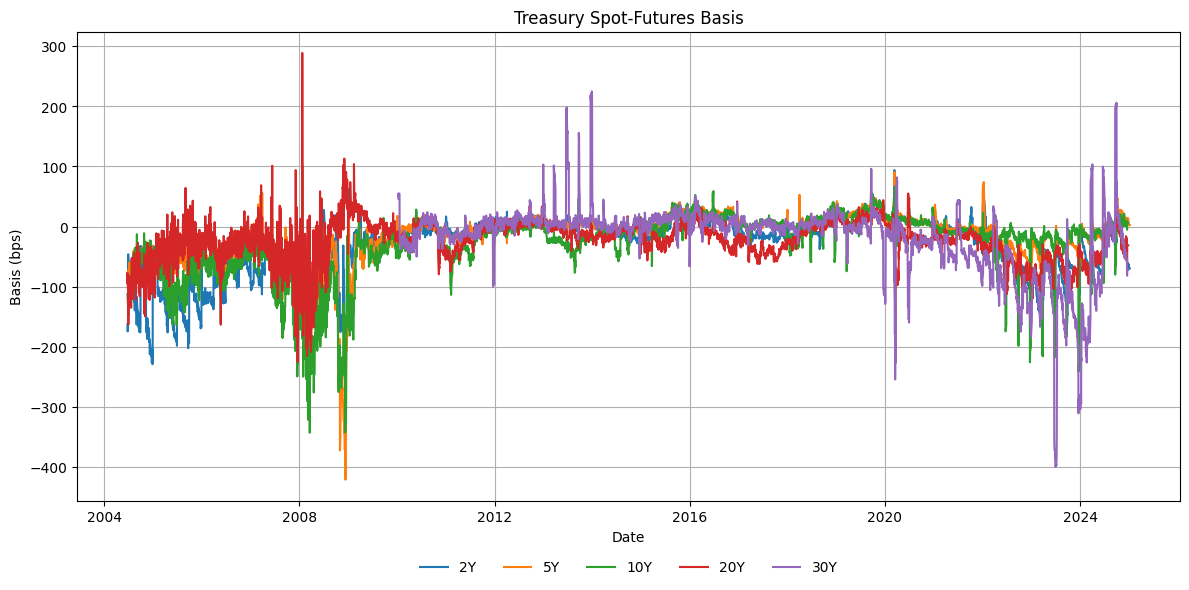
\includegraphics[width=.7\linewidth,height=200pt,width=400pt]{../docs_src/treasury_spot_futures_arbitrage.png}
  \end{tabular}
  \caption{Treasury Spot-Futures Basis (FTSFR Replication)}
  \label{fig:treasury_sf_basis}
\end{figure}


\begin{figure}[h!]
  \centering
  \begin{tabular}{@{}c@{}}
    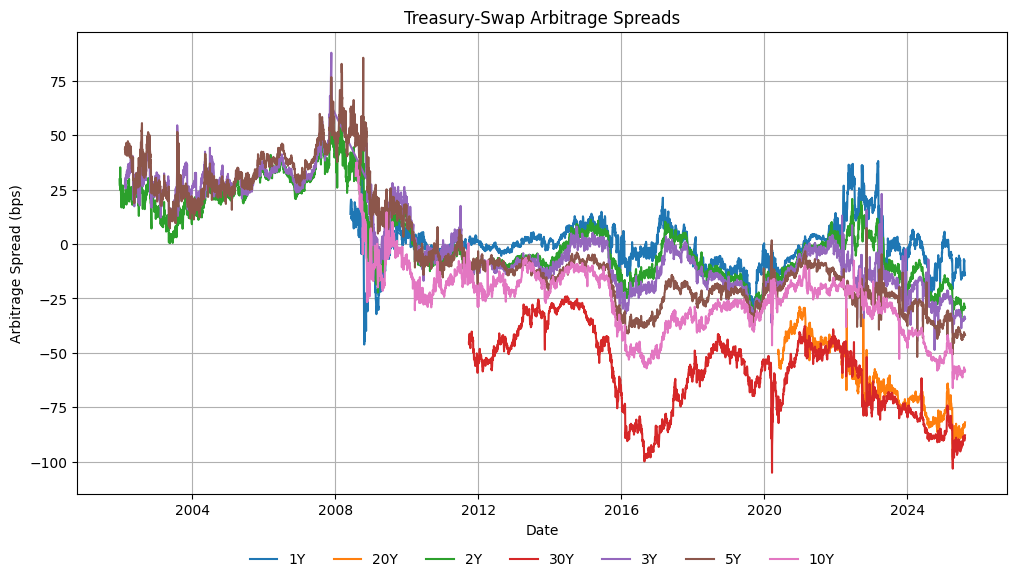
\includegraphics[width=.7\linewidth,height=200pt,width=400pt]{../docs_src/treasury_swap_arbitrage_spreads.png}
  \end{tabular}
  \caption{Treasury Swap Arbitrage spreads.}
  \label{fig:treasury_swap_arbitrage}
\end{figure}


\paragraph{TIPS-Treasury Arbitrage}
Replicating \citet{Fleckenstein2014} as implemented in \citet{Siriwardane2021}, we splice Federal Reserve zero-coupon TIPS yields with Bloomberg constant-maturity inflation-swap rates to create synthetic nominal yields, then difference these against equal-maturity zero-coupon Treasury yields for the 2-, 5-, 10- and 20-year tenors.  We exclude days with missing swap quotes or illiquid TIPS issues, drop outliers beyond the extreme 1\%, and harmonise all series to 17:00 ET closes to obtain a clean daily TIPS-Treasury basis series.

\begin{figure}[h!]
  \centering
  \begin{tabular}{@{}c@{}}
    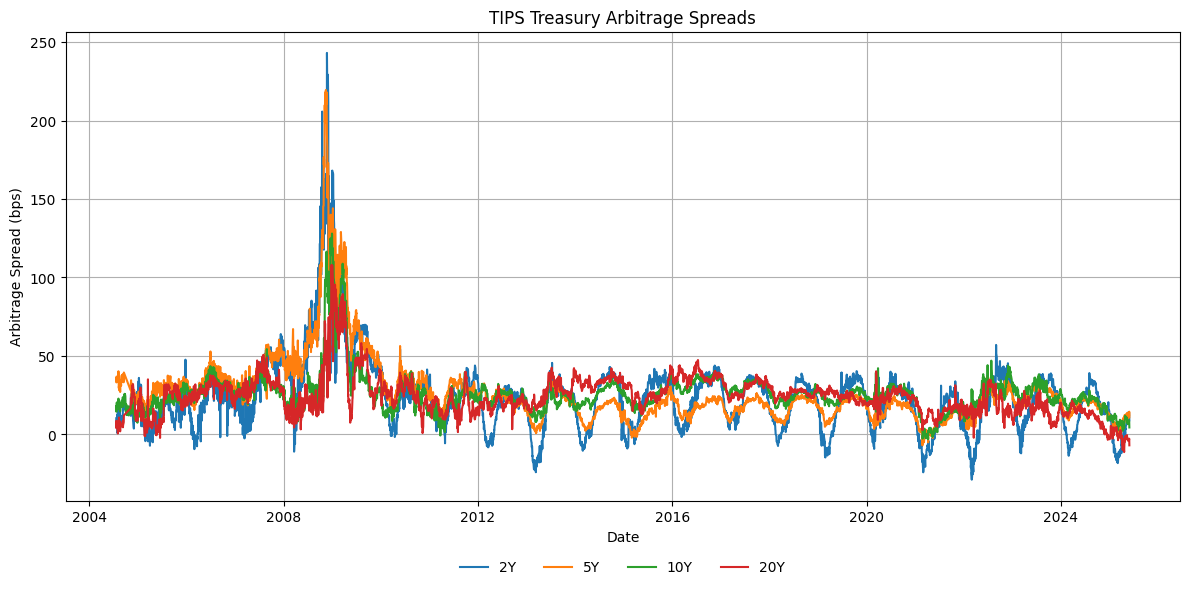
\includegraphics[width=.7\linewidth,height=200pt,width=400pt]{../docs_src/tips_treasury_arbitrage_spreads.png}
  \end{tabular}
  \caption{TIPS-Treasury Arbitrage spreads.}
  \label{fig:tips_treasury_basis}
\end{figure}

\paragraph{CDS-Bond Basis}
% TODO: Check this paragraph.
% we should be doing duration matching, added that in
% i am removing RFR when over 1, representing 100%
% - Vincent
Leveraging the daily Markit pricing files used by \citet{Siriwardane2021}, we link cash bonds to matching single-name CDS and compute the basis after (i) retaining only USD-denominated senior unsecured issues with fixed coupons and 1-10-year maturities, (ii) discarding quotes with prices below 50¢, zero bids, or stale timestamps, and (iii) mapping each bond to a duration-matched CDS par spread via cubic-spline interpolation.  We further exclude callable/convertible structures, winsorise extreme 100\% bases, and require each bond to appear in TRACE's cleaned WRDS dataset to guarantee tradability, yielding a high-quality daily series that mirrors the investment-grade and high-yield bases reported in the original study.


% TODO: Vincent and Alex
% 1. Change y axis label so that it shows percents. Change rfr to "Implied Risk-Free Rate (percent)"
% 2. Get rid of Title in the plot. I can add the title in the LaTeX code myself.
% 3. Get rid of Rating "2", since Rating 2 is the weird hybrid one.
% 4. Rename rating 0 to "High Yield" and rating 1 to "Investment Grade"
\begin{figure}[h!]
  \centering
  \begin{tabular}{@{}c@{}}
    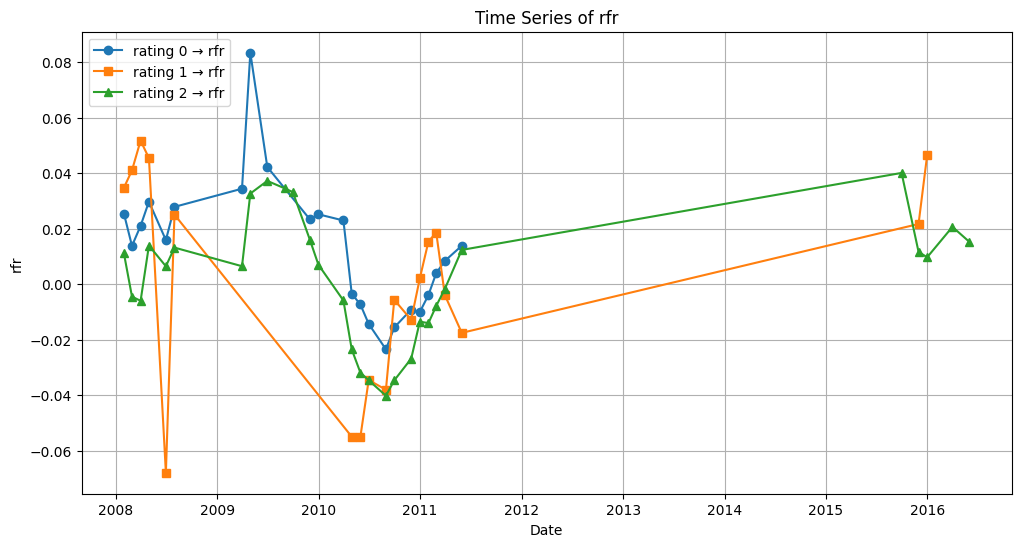
\includegraphics[width=.7\linewidth,height=200pt,width=400pt]{../docs_src/CDS_replicate.png}
  \end{tabular}
  \caption{CDS Arbitrage spreads.}
  \label{fig:cds_basis}
\end{figure}

\paragraph{CIP Arbitrage}
For Covered Interest Parity (CIP) we replicate the G10 series in \citet{Du2018}, merging Bloomberg mid-quotes for spot rates, 3-month forwards, and maturity-matched OIS curves.  Core filters rescale forward points (and invert USD-quoted pairs), synchronise all legs to the 17:00 ET close while dropping holiday or stale quotes, and winsorise the extreme 1\% of annualised spreads with spline interpolation for any missing OIS tenors to remove scaling, timing, and rate-sourcing distortions.

\begin{figure}[h!]
  \centering
  \begin{tabular}{@{}c@{}}
    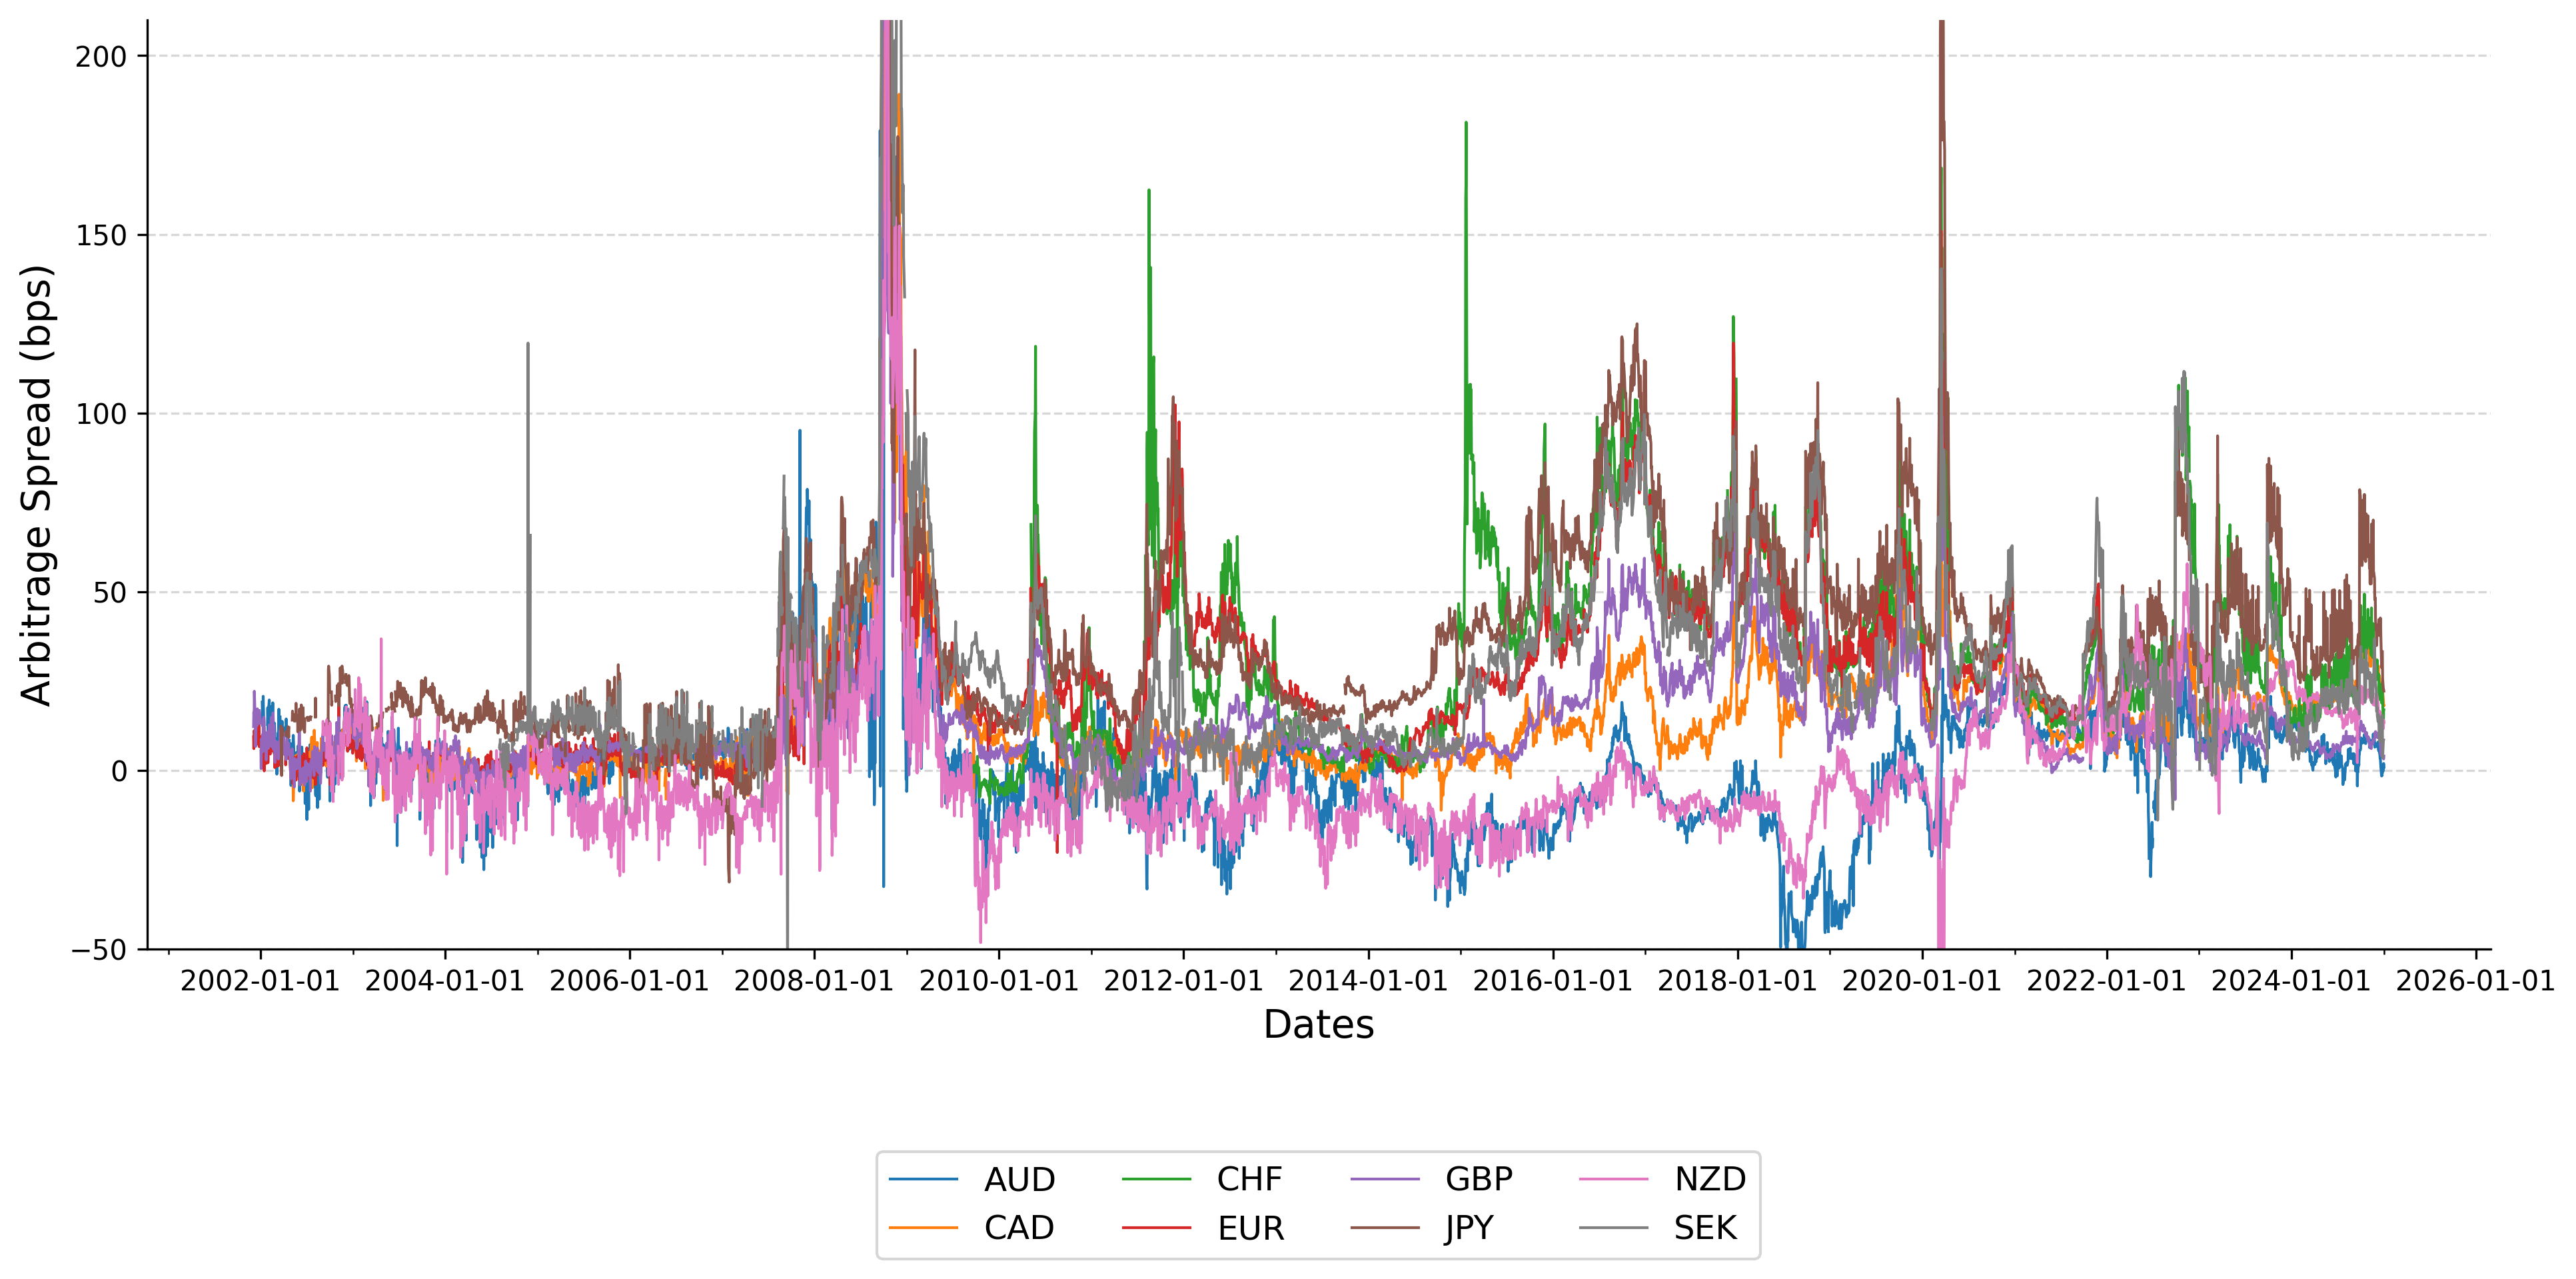
\includegraphics[width=.7\linewidth,height=200pt,width=400pt]{../docs_src/CIP_replicate.png}
  \end{tabular}
  \caption{CIP Arbitrage spreads.}
  \label{fig:cip_basis}
\end{figure}

\paragraph{Spot Futures Arbitrage in Equities}

Following the equity basis recipe of \citet{Hazelkorn2023}, we construct implied forward rates from nearby and first-deferred S\&P 500, Dow Jones, and Nasdaq 100 futures to avoid measurement error from asynchronous spot and futures market closes. We proxy for expected dividends using realized dividends from Bloomberg. The final arbitrage spread is the difference between this futures-implied rate and the 3-month OIS rate, which serves as a clean risk-free benchmark.

\paragraph{Box Arbitrage in Equity Options}
For box spread arbitrage, we follow the methodology of \citet{VanBinsbergen2022} to extract a risk-free rate implied by S\&P 500 (SPX) index options. Their approach uses a cross-sectional regression of put-call price differences on strike prices, which cleverly avoids the need to explicitly estimate dividends. We use their publicly available daily median implied rates and extend the series using their exact methodology on recent minute-level CBOE data. The final arbitrage spread is the difference between this options-implied rate and a maturity-matched OIS rate.

\subsection{Other Financial Data}

\paragraph{Yield Curve}
TODO

\paragraph{Call Report}
TODO

\paragraph{Compustat Panel Data}
TODO




\section{Data Repository Overview}
\label{sec:repository_overview}

% TODO: Provide high-level description of the repository structure and contents
% - Describe the automated data pulling framework
% - List the major categories of data
% - Explain the dual purpose: both for forecasting benchmarks AND for replicating important finance papers
% - Note that replication code for many of these papers was not previously publicly available

\subsection{Repository Architecture}
% Technical structure and automation framework

\subsection{Data Categories}
% Major categories of financial and economic data

\subsection{Data Sources and Access Requirements}
% WRDS, Bloomberg, and other data sources

[Repository overview content to be filled in...]

\section{Replication Results and Validation}
\label{sec:replication}

% TODO: Demonstrate successful replication of all source papers
% - Create comprehensive replication tables
% - Include specific sections for key papers
% - Document any data quality issues discovered
% - Explain any necessary deviations from original methodologies

\subsection{He, Kelly, Manela (2017) Replication}
% Factor loadings and test portfolio returns

\subsection{Siriwardane et al. (2022) Replication}
% Arbitrage spread statistics

\subsection{Individual Dataset Replications}
% Nozawa, Borri & Verdelhan, etc.

[Replication results to be filled in...]

\section{Baseline Forecasting Methodology}
\label{sec:methodology}

% TODO: Define forecasting approach following Monash template
% - Justify choice of error metrics
% - Select baseline forecasting models
% - Define evaluation methodology

\subsection{Error Metrics}
% MASE, sMAPE, RMSE, etc.

\subsection{Baseline Models}
% Traditional, ML, and Deep Learning models
% TODO: Arsh: Add bullet points provide a short 2-3 sentence description of each model. What is the basic idea behind each model? Who developed it? What package are we using to implement it? 

\begin{itemize}
    \item ARIMA: Standard Autoregressive Integrated Moving Average model based on the statsmodel implementation.\cite{Box2013}
    \begin{itemize}
        \item \textbf{Forecasting Type: }Local
        \item \textbf{Package Used: }\texttt{\href{https://unit8co.github.io/darts/generated_api/darts.models.forecasting.arima.html}{darts}}
    \end{itemize}
    \item ETS: We use the Holt-Winter's exponential smoothing model\cite{Winters1960}. % Please add this citation from the URL: https://www.sciencedirect.com/science/article/abs/pii/S0169207003001134
    \begin{itemize}
        \item \textbf{Forecasting Type: }Local
        \item \textbf{Package Used: }\texttt{\href{https://unit8co.github.io/darts/generated_api/darts.models.forecasting.exponential_smoothing.html}{darts}}
    \end{itemize}
    \item Simple Exponential Smoothing: simple exponential moving average on a time-series\cite{Brown2004}.
    \begin{itemize}
        \item \textbf{Forecasting Type: }Local
        \item \textbf{Package Used: }\texttt{\href{https://unit8co.github.io/darts/generated_api/darts.models.forecasting.exponential_smoothing.html}{darts}}
    \end{itemize}
    \item TBATS: Uses Box-Cox transformations, ARMA error corrections and Fourier representations\cite{DeLivera2011}.
    \begin{itemize}
        \item \textbf{Forecasting Type: }Local
        \item \textbf{Package Used: }\texttt{\href{https://unit8co.github.io/darts/generated_api/darts.models.forecasting.sf_tbats.html}{darts}}
    \end{itemize}
    \item Theta: Splits a time-series into multiple Theta lines which are extrpolated separately and their combination is taken as the forecast\cite{Assimakopoulos2000}.
    \begin{itemize}
        \item \textbf{Forecasting Type: }Local
        \item \textbf{Package Used: }\texttt{\href{https://unit8co.github.io/darts/generated_api/darts.models.forecasting.theta.html\#darts.models.forecasting.theta.Theta}{darts}}
    \end{itemize}
    \item Prophet: decomposable time-series model similar to Generalized Additive Model(GAM) developed by Facebook\cite{Taylor2018}.
    \begin{itemize}
        \item \textbf{Forecasting Type: }Local
        \item \textbf{Package Used: }\texttt{\href{https://unit8co.github.io/darts/generated_api/darts.models.forecasting.prophet_model.html}{darts}}
    \end{itemize}
    \item PR (Pooled Regression): Generic gaussian linear model\cite{Trapero2015}
    \begin{itemize}
        \item \textbf{Forecasting Type: }Global
        \item \textbf{Package Used: }\texttt{\href{https://unit8co.github.io/darts/generated_api/darts.models.forecasting.sklearn_model.html\#darts.models.forecasting.sklearn_model.SKLearnModel}{darts}} and \texttt{\href{https://scikit-learn.org/stable/modules/generated/sklearn.linear_model.TweedieRegressor.html\#sklearn.linear_model.TweedieRegressor}{scikit-learn}}
    \end{itemize}
    \item CatBoost: Gradient boosting algorithm for dealing with categorical data and a leaf value calculation trick which reduces overfitting\cite{Prokhorenkova}.
    \begin{itemize}
        \item \textbf{Forecasting Type: }Global
        \item \textbf{Package Used: }\texttt{\href{https://unit8co.github.io/darts/generated_api/darts.models.forecasting.catboost_model.html}{darts}}
    \end{itemize}
    \item FFNN (Feed-Forward Neural Network): Simple neural network which is a collection of weight tensors with activation functions in between\cite{Goodfellow2016}.
    \begin{itemize}
        \item \textbf{Forecasting Type: }Global
        \item \textbf{Package Used: }\texttt{\href{https://ts.gluon.ai/stable/api/gluonts/gluonts.torch.model.simple_feedforward.html}{gluonts}} with \texttt{torch} backend
    \end{itemize}
    \item Transformer: A deep network architecture utilising attention mechanisms for deducing dependencies in the input and the output\cite{Vaswani2017}.
    \begin{itemize}
        \item \textbf{Forecasting Type: }Global
        \item \textbf{Package Used: }\texttt{\href{https://unit8co.github.io/darts/generated_api/darts.models.forecasting.transformer_model.html}{darts}}
    \end{itemize}
    \item DeepAR: An Autoregressive Recurrent Neural Network(RNN) with Long Short-Term Memory(LSTM).\cite{Salinas2020}
    \begin{itemize}
        \item \textbf{Forecasting Type: }Global
        \item \textbf{Package Used: }\texttt{\href{https://ts.gluon.ai/stable/api/gluonts/gluonts.torch.model.deepar.module.html}{gluonts}} with \texttt{torch} backend
    \end{itemize}
    \item WaveNet: Dilated deep neural network employing convolution layers. Originally made to generate sound waveforms\cite{Oord2016} but adapted to use in forecasting. % PLEASE ADD CITATION FROM URL: https://arxiv.org/abs/1703.04691
    \begin{itemize}
        \item \textbf{Forecasting Type: }Global
        \item \textbf{Package Used: }\texttt{\href{https://ts.gluon.ai/stable/api/gluonts/gluonts.torch.model.wavenet.html}{gluonts}} with \texttt{torch} backend
    \end{itemize}
    \item D-Linear: Transformer-based deep model which is a combination of a decomposition scheme with linear layers\cite{Zeng2022}.
    \begin{itemize}
        \item \textbf{Forecasting Type: }Global
        \item \textbf{Package Used: }\texttt{\href{https://unit8co.github.io/darts/generated_api/darts.models.forecasting.dlinear.html}{darts}}
    \end{itemize}
    \item N-Linear: Transformer-based deep model which addresses distribution shifts in the dataset by using a normalization trick\cite{Zeng2022}.
    \begin{itemize}
        \item \textbf{Forecasting Type: }Global
        \item \textbf{Package Used: }\texttt{\href{https://unit8co.github.io/darts/generated_api/darts.models.forecasting.nlinear.html}{darts}}
    \end{itemize}
    \item N-BEATS: Deep neural network with fully-connected layers along with residual links\cite{Oreshkin2020}.
    \begin{itemize}
        \item \textbf{Forecasting Type: }Global
        \item \textbf{Package Used: }\texttt{\href{https://unit8co.github.io/darts/generated_api/darts.models.forecasting.nbeats.html}{darts}}
    \end{itemize}
    \item N-HiTS: Enhances N-BEATS by using multi-rate data sampling and multi-scale interpolation\cite{Challu2022}.
    \begin{itemize}
        \item \textbf{Forecasting Type: }Global
        \item \textbf{Package Used: }\texttt{\href{https://unit8co.github.io/darts/generated_api/darts.models.forecasting.nhits.html\#darts.models.forecasting.nhits.NHiTSModel}{darts}}
    \end{itemize}
    \item Autoformer: Transformer-based deep network employing decomposition and Auto-Correlation\cite{Wu2021}.
    \begin{itemize}
        \item \textbf{Forecasting Type: }Global
        \item \textbf{Package Used: }Nixtla's \texttt{\href{https://nixtlaverse.nixtla.io/neuralforecast/models.autoformer.html}{neuralforecast}}
    \end{itemize}
    \item Informer: Transformer-based architecture using a ProbSparse self-attention mechanism and a generative-style decoder among other techniques\cite{Zhou2020}.
    \begin{itemize}
        \item \textbf{Forecasting Type: }Global
        \item \textbf{Package Used: }Nixtla's \texttt{\href{https://nixtlaverse.nixtla.io/neuralforecast/models.informer.html}{neuralforecast}}
    \end{itemize}
    \item PatchTST: Transformer-based model breaking a time series into a collection of patches used as tokens and utilises channel independence\cite{Nie2022}.
    \begin{itemize}
        \item \textbf{Forecasting Type: }Global
        \item \textbf{Package Used: }\texttt{\href{https://ts.gluon.ai/stable/api/gluonts/gluonts.torch.model.patch_tst.html}{gluonts}} with \texttt{torch} backend
    \end{itemize}
    \item Temporal Fusion Transformer: Transformer-based model employing recurrent layers and self-attention layers with a focus on interpretablility\cite{Lim2021}
    \begin{itemize}
        \item \textbf{Forecasting Type: }Global
        \item \textbf{Package Used: }\texttt{\href{https://ts.gluon.ai/stable/api/gluonts/gluonts.torch.model.tft.module.html}{gluonts}} with \texttt{torch} backend
    \end{itemize}
    \item Time-series Dense Encoder(TiDE): Multi-layer perceptron based architecture utilising encoder and decoder blocks\cite{Das2023a}.
    \begin{itemize}
        \item \textbf{Forecasting Type: }Global
        \item \textbf{Package Used: }\texttt{\href{https://unit8co.github.io/darts/generated_api/darts.models.forecasting.tide_model.html}{darts}}
    \end{itemize}
    \item TimesFM: Pre-trained transformer-based decoder-only deep model utilising patches similar to PatchTST\cite{Das2023}.
    \begin{itemize}
        \item \textbf{Forecasting Type: }Global
        \item \textbf{Package Used: }\texttt{\href{https://github.com/google-research/timesfm}{timesfm}} python package
    \end{itemize}
\end{itemize}

\subsection{Evaluation Framework}
% Train/test splits, structural breaks, etc.

[Methodology content to be filled in...]

\section{Baseline Results and Analysis}
\label{sec:results}

% TODO: Present comprehensive forecasting results across all datasets
% - Create results tables in exact same format as Monash paper
% - Analyze patterns in results
% - Compare with Monash findings where applicable
% - Discuss implications for practitioners

\subsection{Overall Performance}
% Summary tables across all datasets

We present comprehensive forecasting results across all datasets and models using two primary error metrics: Mean Absolute Scaled Error (MASE) and Root Mean Square Error (RMSE). MASE provides scale-free comparison across different time series, while RMSE captures the magnitude of forecasting errors in original units.

Table~\ref{tab:mase_results} shows MASE results for all model-dataset combinations. The table is organized with datasets as rows and forecasting models as columns, allowing for easy comparison of model performance within each dataset and identification of datasets that present particular challenges for forecasting.

% MASE Results by Dataset and Model
% Generated automatically by create_results_tables2.py

\begin{table}[htbp]
\centering
\caption{MASE Results by Dataset and Model}
\label{tab:mase_results}
\scriptsize
\setlength{\tabcolsep}{2pt}
\renewcommand{\arraystretch}{0.85}
\begin{tabular}{@{}l@{\hspace{2pt}}@{\hspace{1pt}}r@{\hspace{1pt}}@{\hspace{1pt}}r@{\hspace{1pt}}@{\hspace{1pt}}r@{\hspace{1pt}}@{\hspace{1pt}}r@{\hspace{1pt}}@{\hspace{1pt}}r@{\hspace{1pt}}@{\hspace{1pt}}r@{\hspace{1pt}}@{\hspace{1pt}}r@{\hspace{1pt}}@{\hspace{1pt}}r@{\hspace{1pt}}@{\hspace{1pt}}r@{\hspace{1pt}}@{\hspace{1pt}}r@{\hspace{1pt}}@{\hspace{1pt}}r@{\hspace{1pt}}@{\hspace{1pt}}r@{\hspace{1pt}}@{\hspace{1pt}}r@{\hspace{1pt}}@{}}
\toprule
 & ARIMA & ETS & Theta & DLinear & DeepAR & KAN & NBEATS & NHITS & NLinear & Naive & SN & TiDE & Transformer \\
\midrule
\multicolumn{14}{l}{\textbf{Basis Spreads}} \\
CDS-Bond & 1.48 & 1.01 & 1.01 & 1.57 & 1.24 & 0.82 & 0.83 & 0.90 & 0.99 & 1.01 & 0.94 & 0.83 & 0.76 \\
CIP & 0.66 & 0.60 & 0.60 & 1.02 & 0.98 & 0.56 & 0.59 & 0.58 & 0.66 & 0.60 & 0.64 & 0.67 & 0.92 \\
TIPS-Treasury & 1.09 & 0.65 & 0.65 & 1.12 & 1.10 & 0.63 & 0.65 & 0.65 & 0.67 & 0.65 & 0.61 & 0.71 & 1.00 \\
Treasury-SF & 1.43 & 1.43 & 1.43 & 1.92 & 1.95 & 1.90 & 1.74 & 1.58 & 1.54 & 1.43 & 1.79 & 1.85 & 1.96 \\
Treasury-Swap & 2.87 & 1.75 & 1.75 & 3.29 & 3.61 & 2.98 & 2.02 & 2.00 & 1.74 & 1.75 & 1.74 & 2.46 & 3.41 \\
\midrule
\multicolumn{14}{l}{\textbf{Returns (Portfolios)}} \\
CDS Portfolio & 1.69 & 0.82 & 0.84 & 885.21 & 11.17 & 3.34 & 10.67 & 196.65 & 688.65 & 1.05 & 1.05 & 292.36 & 367.88 \\
Corporate Portfolio & 1.16 & 1.16 & 1.15 & 13.93 & 1.16 & 1.18 & 1.22 & 2.60 & 9.75 & 1.19 & 1.19 & 4.82 & 5.29 \\
FF25 Size-BM & 0.99 & 1.17 & 1.17 & 16.77 & 1.04 & 0.99 & 1.26 & 4.32 & 12.98 & 1.17 & 1.17 & 6.26 & -- \\
FF25 Size-Inv & 1.01 & 1.36 & 1.36 & 18.60 & 1.06 & 1.00 & 1.47 & 4.23 & 14.41 & 1.36 & 1.36 & 6.57 & -- \\
FF25 Size-Op & 1.02 & 1.38 & 1.38 & 18.49 & 1.07 & 1.02 & 1.49 & 4.22 & 14.34 & 1.38 & 1.38 & 6.54 & -- \\
HKM All Factor & 4.52 & 3.81 & 4.78 & 16.50 & 19.30 & 4.24 & 5.38 & 7.48 & 12.50 & 4.54 & 4.54 & 8.38 & 20.96 \\
HKM Daily Factor & 4.91 & 4.93 & 4.93 & 65.55 & 98.50 & 7.05 & 7.50 & 21.30 & 46.03 & 4.93 & 4.93 & 23.05 & 83.45 \\
HKM Monthly Factor & 10.96 & 12.73 & 11.09 & 19.41 & 19.60 & 5.63 & 9.05 & 12.43 & 19.01 & 11.51 & 11.51 & 7.71 & 21.55 \\
Treasury Portfolio & 0.58 & 0.58 & 0.62 & 37.18 & 0.64 & 0.66 & 0.79 & 7.31 & 25.96 & 0.59 & 0.59 & 13.16 & 26.54 \\
\midrule
\multicolumn{14}{l}{\textbf{Returns (Disaggregated)}} \\
CDS Contract & 2.12 & 1.88 & 1.88 & 68.71 & 2.12 & 1.95 & 2.06 & 20.36 & 59.29 & 1.88 & 1.88 & 23.57 & 30.89 \\
CJS Option & 1.42 & 1.26 & 1.26 & 11.20 & 1.65 & 0.90 & 1.27 & 3.07 & 9.24 & 1.26 & 1.26 & 4.50 & 10.26 \\
CRSP Stock & 4.36 & 6.58 & 6.65 & 6.35 & 4.51 & 4.43 & 5.65 & 6.59 & 2.81 & 6.58 & 6.58 & 3.66 & 10.99 \\
CRSP Stock (ex-div) & 4.35 & 6.57 & 6.64 & 6.34 & 4.47 & 4.38 & 5.49 & 6.56 & 2.79 & 6.57 & 6.57 & 3.51 & 10.95 \\
Commodity & 0.74 & 0.80 & 0.80 & 2.51 & 0.75 & 0.75 & 0.77 & 0.93 & 1.68 & 0.80 & 0.80 & 0.97 & 1.96 \\
Corporate Bond & 1.03 & 1.13 & 1.21 & 10.44 & 0.99 & 0.97 & 1.17 & 1.89 & 9.61 & 1.16 & 1.16 & 5.33 & 5.32 \\
FX & 18.85 & 18.85 & 18.85 & 19.62 & 20.48 & 20.90 & 19.68 & 20.45 & 19.86 & 18.85 & 18.85 & 18.84 & 18.92 \\
HKM Option & 1.74 & 1.35 & 1.35 & 13.41 & 1.92 & 1.00 & 1.51 & 3.52 & 11.04 & 1.35 & 1.35 & 5.30 & 12.23 \\
Treasury Bond & 0.48 & 0.51 & 0.61 & 61.58 & 0.61 & 0.80 & 0.62 & 5.91 & 28.77 & 0.48 & 0.48 & 21.82 & 25.03 \\
\midrule
\multicolumn{14}{l}{\textbf{Other}} \\
BHC Cash Liquidity & 3.16 & 2.42 & 2.38 & 16.12 & 3.14 & 2.27 & 2.38 & 3.02 & 11.50 & 2.32 & 2.44 & 5.26 & 5.37 \\
BHC Leverage & 10.22 & 2.97 & 3.04 & 17.80 & 17.50 & 2.33 & 2.64 & 2.68 & 4.16 & 2.89 & 2.99 & 7.12 & 14.25 \\
Bank Cash Liquidity & 999.00 & 999.00 & 999.00 & 999.00 & 999.00 & 999.00 & 999.00 & 999.00 & 999.00 & 999.00 & 999.00 & 999.00 & 999.00 \\
Bank Leverage & 2.69 & 2.01 & 2.05 & 10.79 & 10.46 & 4.91 & 1.95 & 1.99 & 2.16 & 1.87 & 2.06 & 4.04 & 9.05 \\
Treasury Yield Curve & 8.69 & 8.69 & 8.69 & 23.57 & 13.86 & 8.80 & 9.98 & 10.64 & 8.86 & 8.69 & 8.93 & 11.30 & -- \\
\bottomrule
\end{tabular}
\vspace{0.05cm}
\noindent {\scriptsize \textbf{Note:} Values show Mean Absolute Scaled Error (MASE). Lower values indicate better performance. -- indicates missing results.}
\end{table}


Figure~\ref{fig:mase_heatmap} provides a visual representation of the MASE results from Table~\ref{tab:mase_results}. The color-coded heatmap makes it easy to identify patterns in model performance across different dataset types, with cooler colors (blues) indicating better performance and warmer colors (reds) indicating poorer performance.

\begin{figure}[htbp]
\centering
\includegraphics[width=\textwidth]{../_output/forecasting2/mase_heatmap.png}
\caption{MASE Results Heatmap by Dataset and Model. Cooler colors (blue) indicate better performance (lower error), while warmer colors (red) indicate poorer performance (higher error). Color scaling is capped at the 90th percentile to highlight differences among the majority of values; extreme outliers are marked with asterisks (*) and show actual values.}
\label{fig:mase_heatmap}
\end{figure}

Table~\ref{tab:rmse_results} presents the corresponding RMSE results using the same organization. While MASE provides scale-free comparisons, RMSE offers insights into the actual magnitude of forecasting errors, which can be particularly relevant for risk management applications.

% RMSE Results by Dataset and Model
% Generated automatically by create_results_tables2.py

\begin{table}[htbp]
\centering
\caption{RMSE Results by Dataset and Model}
\label{tab:rmse_results}
\scriptsize
\setlength{\tabcolsep}{1.5pt}
\renewcommand{\arraystretch}{0.9}
\begin{tabular}{@{}lrrrrrrrrrr@{}}
\toprule
 & HistAvg & ARIMA & Theta & DeepAR & NBEATS & NHITS & DLinear & NLinear & TiDE & KAN \\
\midrule
\multicolumn{11}{l}{\textbf{Returns (Portfolios)}} \\
CDS Portfolio & -- & 0.00 & \textbf{0.00} & -- & -- & -- & -- & -- & -- & -- \\
Corporate Portfolio & 0.03 & 0.03 & 0.03 & 0.03 & 0.03 & 0.02 & 0.02 & 0.02 & \textbf{0.02} & 0.03 \\
SPX Options Portfolios & \textbf{0.03} & 0.04 & 0.04 & 0.04 & 0.03 & 0.03 & 0.03 & 0.03 & 0.03 & 0.03 \\
Treasury Portfolio & -- & \textbf{0.01} & 0.01 & -- & -- & -- & -- & -- & -- & -- \\
\midrule
\multicolumn{11}{l}{\textbf{Other}} \\
HKM All Factor & 45.45 & \textbf{41.87} & 43.57 & 104.93 & 98.60 & 85.21 & 105.52 & 106.78 & 105.53 & 95.90 \\
HKM Monthly Factor & 44.21 & 22.10 & \textbf{20.80} & 70.65 & 1544.49 & 262.32 & 172.93 & 196.16 & 153.58 & 363.03 \\
\bottomrule
\end{tabular}
\vspace{0.1cm}

\noindent {\scriptsize \textbf{Note:} Values show Root Mean Square Error (RMSE). Lower values indicate better performance. -- indicates missing results.}
\end{table}


Figure~\ref{fig:rmse_heatmap} visualizes the RMSE results, complementing the numerical table with a clear color-coded representation of relative model performance across all datasets.

\begin{figure}[htbp]
\centering
\includegraphics[width=\textwidth]{../_output/forecasting2/rmse_heatmap.png}
\caption{RMSE Results Heatmap by Dataset and Model. Colors are capped at the 90th percentile to highlight performance differences across the majority of datasets, with extreme outliers marked with asterisks (*). The visualization reveals models that consistently perform well and datasets that pose particular forecasting challenges.}
\label{fig:rmse_heatmap}
\end{figure}

\subsection{Results by Asset Class}
% Detailed analysis for each asset class

\subsection{Results by Model Type}
% Comparison of traditional vs ML vs DL approaches

\subsection{Comparison with Monash Benchmarks}
% How financial data differs from general time series

[Results content to be filled in...]

\section{Implementation and Usage}
\label{sec:implementation}

% TODO: Explain technical architecture and usage
% - Document the automation framework
% - Provide clear usage instructions
% - Explain design decisions
% - Include code examples

\subsection{Installation and Setup}
% Requirements and installation process

\subsection{Data Pipeline Architecture}
% dodo.py and automation framework

\subsection{Adding New Datasets}
% Extensibility and contribution guidelines

[Implementation content to be filled in...]

\section{Reproducibility}
\label{sec:reproducibility}

% TODO: Ensure full reproducibility of all results
% - Document exact data vintage used
% - Provide checksums for all processed datasets
% - Include random seeds
% - Detail computational environment

[Reproducibility content to be filled in...]

\section{Conclusions and Future Work}
\label{sec:conclusion}

% TODO: Summarize contributions and outline future extensions
% - Recap main contributions
% - Discuss potential additional datasets
% - Propose enhanced forecasting methods
% - Suggest infrastructure improvements
% - Note community contribution guidelines

[Conclusion content to be filled in...]

\section*{Acknowledgments}

We would like to thank the following individuals. With their permission, we have adapted and used pieces of their code in this repository: Om Mehta and Kunj Shah for their replication of the Covered Interest Rate Parity (CIP) arbitrage spreads; Kyle Parran and Duncan Park for their replication of commodity futures returns; Haoshu Wang and Guanyu Chen for their replication of the Treasury Spot-Futures basis; Arsh Kumar and Raiden Egbert for their replication of the Treasury Swap basis; and Bailey Meche and Raul Renteria for their replication of the TIPS-Treasury basis.


% TODO: Add additional acknowledgments

\begin{appendices}

\section{Data Cleaning Procedures and Replications}
\label{app:data_cleaning_and_replications}
% Detailed descriptions of each dataset

\subsection{Asset Class Datasets}
\label{sec:asset_classes}

% TODO: Document each asset class dataset with its canonical cleaning method
% For EACH asset class, create a subsection that includes:
% - Which specific paper's cleaning method is being replicated
% - Why this dataset/asset class is important for macro-finance
% - Key cleaning decisions and their justifications
% - Summary statistics that match the original paper (proving correct replication)

Following \cite{He2017}, we include comprehensive datasets across multiple asset classes, each cleaned according to canonical methods from the academic literature.

\subsubsection{Equity Markets}
\label{sec:equity}
% Fama-French 25 portfolios and CRSP universe
% Explain exclusion of small stocks, ADRs, etc. following Fama-French (1993)

The equity dataset follows \cite{Fama1993}, whose cleaning methodology has 
become the canonical approach in asset pricing research, establishing the 
foundation for thousands of subsequent studies. The essential data transformations 
in Fama-French are critical for avoiding common pitfalls in equity research. 
First, their precise definition of book equity carefully accounts for balance 
sheet complexities: book value of stockholders' equity plus deferred taxes and 
investment tax credits minus the book value of preferred stock, with 
a hierarchical approach to valuing preferred stock (redemption, liquidation, or 
par value). This standardization is crucial because inconsistent book equity 
definitions can dramatically alter value factor exposures and lead to spurious 
results. Second, their exclusion criteria eliminate securities that would 
contaminate standard equity analysis: ADRs (which reflect foreign market dynamics), 
REITs and units of beneficial interest (which have fundamentally different 
cash flow structures), and firms with negative book equity 
(which represent financial distress and behave differently from normal equity 
securities). Finally, using NYSE breakpoints for size and book-to-market 
sorting prevents the results from being dominated by the numerous small 
NASDAQ and AMEX stocks that entered the sample after 1972. These seemingly 
technical choices have profound impacts: studies that deviate from these conventions 
often find dramatically different results, and the stability of the size and value 
effects across decades of out-of-sample testing validates these careful data 
handling procedures. By open-sourcing code that implements these exact 
transformations, we enable researchers to avoid the numerous subtle errors that 
can arise when attempting to reconstruct this canonical dataset from raw CRSP data.

The following figures show summary statistics of the CRSP universe of stocks, 
including the average returns of all stocks for each given date (Figure 6) 
and the average three month rolling standard deviation for a given date (Figure 7).
The earlier years of the dataset are dominated by small stocks, 
which have higher average returns and higher volatility, while the later years of 
the dataset is more diverse, leading to lower average returns and lower volatility.

\begin{figure}[h!]
  \centering
  \begin{tabular}{@{}c@{}}
    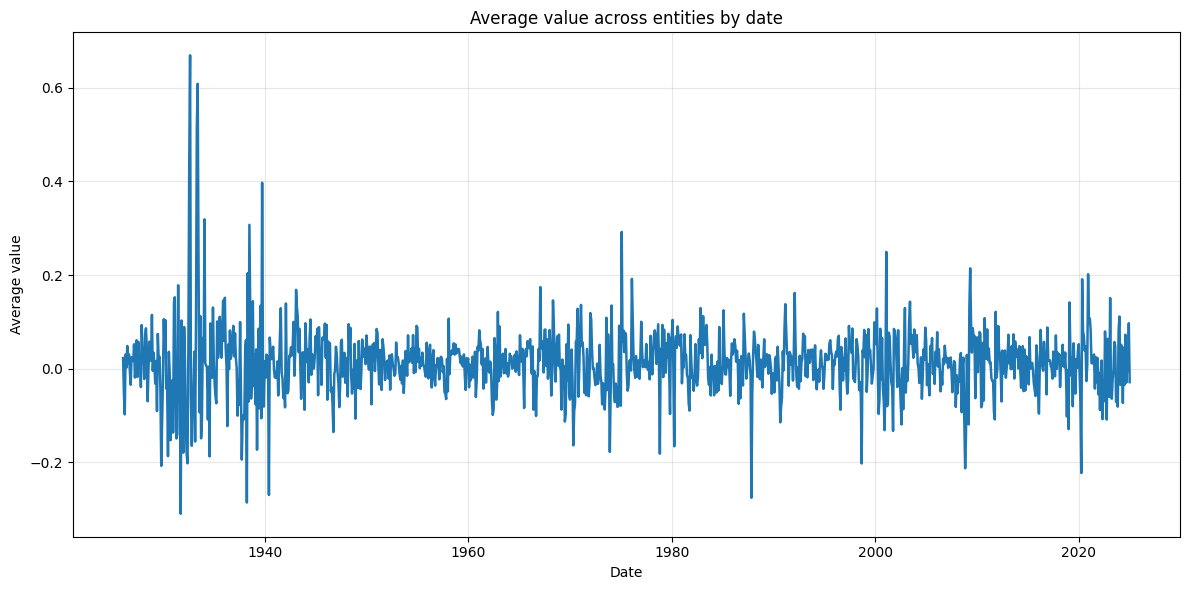
\includegraphics[width=.7\linewidth,height=200pt,width=400pt]{../docs_src/daily_avg_returns_CRSP_COMPU.png}
  \end{tabular}
  \caption{Average returns of all stocks for a given date}
  \label{fig:avg_returns_crsp}
\end{figure}

\begin{figure}[h!]
  \centering
  \begin{tabular}{@{}c@{}}
    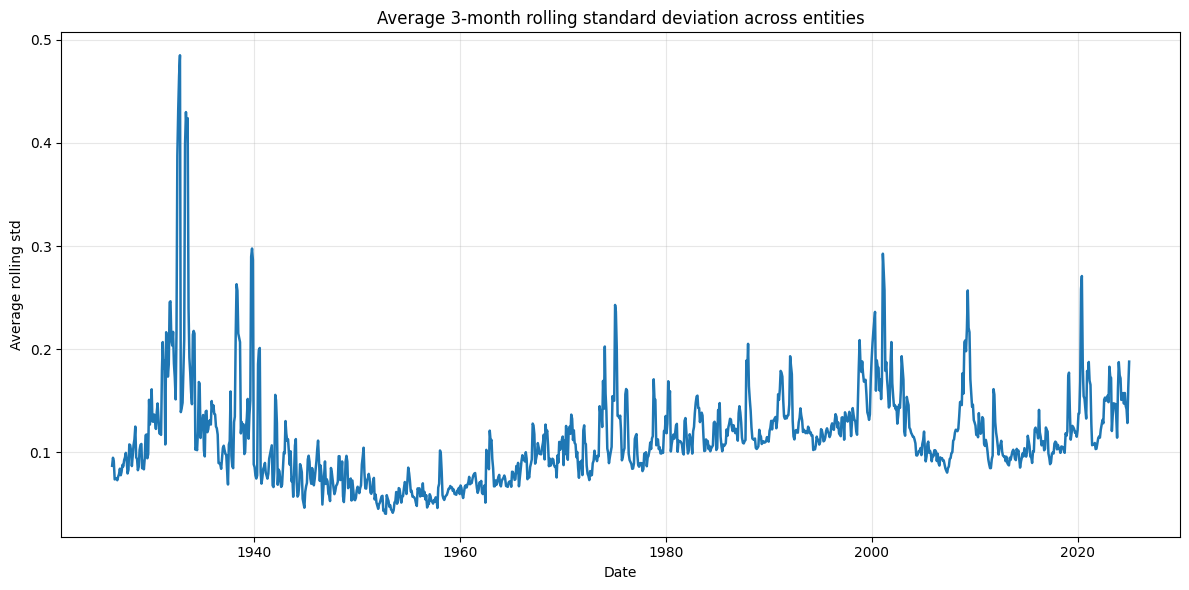
\includegraphics[width=.7\linewidth,height=200pt,width=400pt]{../docs_src/Average_three_month_rolling_std.png}
  \end{tabular}
  \caption{Average three month rolling standard deviation for a given date}
  \label{fig:avg_rolling_std_crsp}
\end{figure}

\FloatBarrier


\subsubsection{US Treasuries}
\label{sec:treasuries}
% CRSP maturity-sorted portfolios Treasuries

The US Treasury dataset follows \cite{Gurkaynak2007}, whose methodology has become the canonical approach for constructing Treasury yield curves and returns. This framework forms the foundation for the Federal Reserve's own yield curve estimates and underpins numerous studies in fixed income research.

The essential data transformations address critical issues unique to government bond markets. First, the restriction to noncallable bonds and notes—excluding bills and other security types—is fundamental. Callable bonds embed optionality that contaminates pure interest rate risk measurement. For example, a bond trading at a premium with an embedded call option will exhibit negative convexity and compressed returns, distorting any analysis of term structure dynamics.

Second, the dataset focuses on bonds with remaining maturities between 0 and 5 years. This reflects market microstructure realities: bonds with longer maturities often suffer from illiquidity and fragmented trading, whereas the 0–5 year segment represents the most actively traded Treasury securities where price discovery is most efficient.

Third, the careful handling of accrued interest in return calculations is essential. Unlike equities, bond prices are quoted as clean prices (excluding accrued interest), but return calculations must incorporate coupon payments. Failing to account for this leads to dramatic miscalculations of returns, especially around coupon payment dates.

Fourth, a requirement for complete price and maturity information ensures that bonds with sporadic trading activity or ambiguous terms are excluded. This prevents noise from entering the yield curve estimation and return construction process.

Fifth, the use of month-end observations for portfolio aggregation avoids substantial day-of-month effects in Treasury markets. These effects arise from auction cycles, end-of-month portfolio rebalancing, and futures contract rolls, all of which can distort return measures if not properly controlled.

These seemingly technical choices have profound implications. Studies that use the full set of Treasury data without these filters often report spurious term premia and unstable factor loadings. In contrast, the Gürkaynak, Sack, and Wright methodology yields stable estimates that closely match dealer quotes and futures-implied yields.

By open-sourcing the exact implementation of these filters, we enable researchers to avoid common errors such as including Treasury STRIPS (which have different tax treatment), century bonds (which have unique clienteles), or inflation-indexed securities (which embed inflation risk) in nominal Treasury analysis.

A comparison of the treasury bond returns dataset with the FTSFR dataset is shown in Figure \ref{fig:us_treasury_returns_comparison}.

\begin{figure}[h]
  \centering
  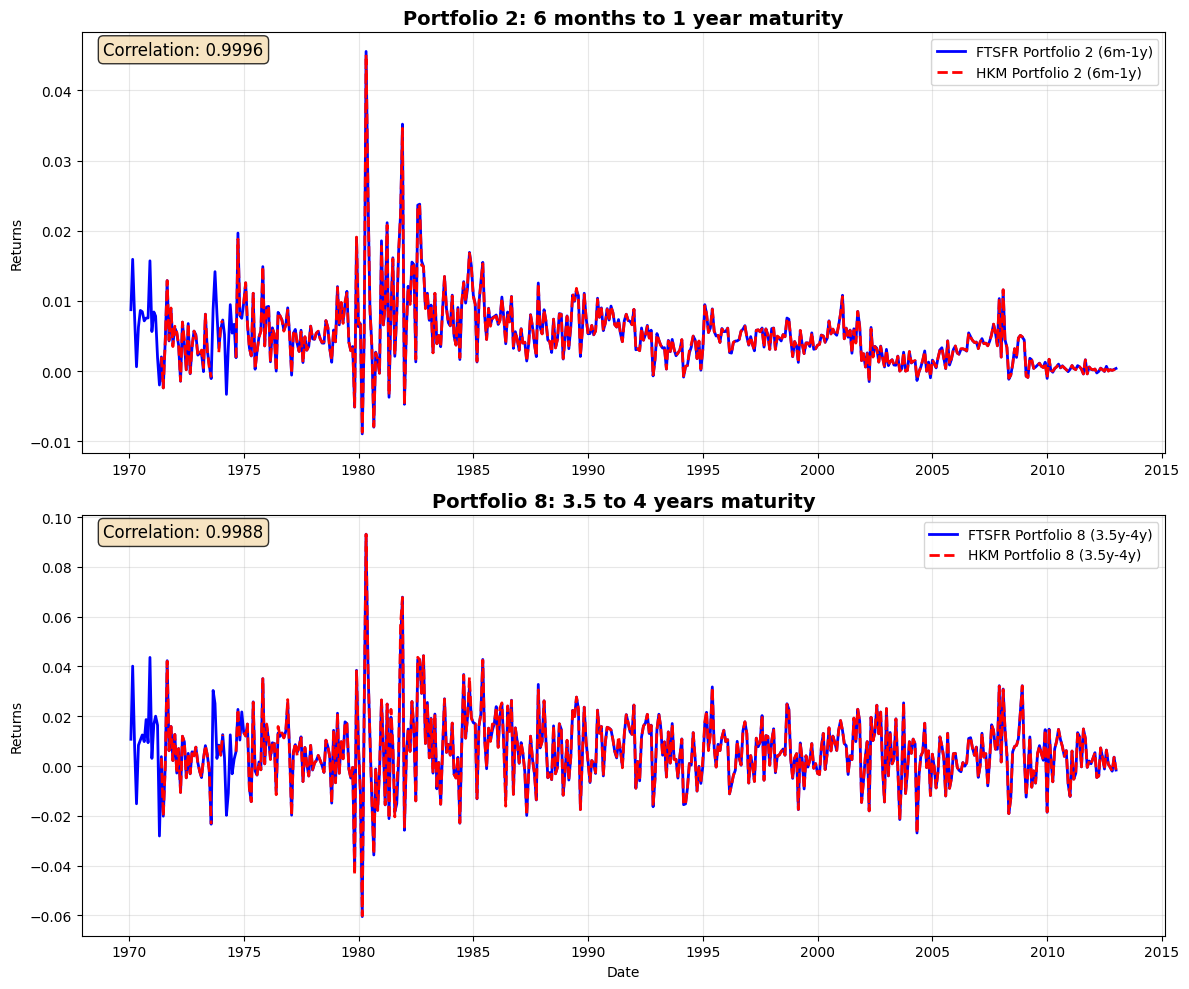
\includegraphics[width=0.8\textwidth]{../docs_src/us_treasury_compare.png}
  \caption{Comparison of He, Kelly, and Manela (2017) treasury bond returns dataset with FTSFR dataset}
  \label{fig:us_treasury_returns_comparison}
\end{figure}

\subsubsection{Corporate Bonds}
\label{sec:corporate_bonds}

% Nozawa (2017) yield-spread sorted portfolios
The corporate bond returns data is sourced from the TRACE (Trade Reporting and Compliance Engine) dataset, available at openbondassetpricing.com, and follows the methodology outlined in Nozawa (2017). This dataset incorporates several key elements to ensure accuracy and relevance. First, it includes market microstructure adjustments to correct for noise and enhance the reliability of bond prices and returns. It also applies stringent data filters, such as including only U.S.-domiciled firms and excluding private placements and convertible bonds. The dataset covers corporate bonds with sufficient outstanding amounts and complete information, and includes essential fields such as MMN-adjusted clean prices, amount outstanding, monthly returns, and credit spreads.

The cleaning and standardization procedure adheres to the rigorous framework established by Nozawa (2017) and adopted by He, Kelly, and Manela (HKM). In terms of bond selection, floating rate bonds and those with put or convertible features are excluded, although callable bonds are retained. Bonds are removed if their prices exceed matched Treasury prices or fall below \$0.01 per \$1 face value. For return processing, return reversals are eliminated if the product of adjacent returns is less than -0.04, and monthly returns are computed to avoid assumptions about reinvestment. In synthetic Treasury construction, Treasury bonds with identical cash flow structures are constructed for each corporate bond using Federal Reserve constant-maturity yield data. Excess returns and credit spreads are then calculated in price terms rather than yield spreads.

For portfolio construction, bonds are sorted into deciles based on credit spreads for each date. Value-weighted portfolio returns are computed using bond values—defined as the product of MMN-adjusted clean price and amount outstanding—as weights. To ensure data quality, defaults are verified using Moody's Default Risk Service, while CRSP and Compustat data supplement the equity and accounting information. Callable bonds are also incorporated into regression models using fixed effects.

The final output is a dataset containing monthly corporate bond portfolio returns sorted by credit spread deciles, making it well-suited for credit risk analysis and for benchmarking against other bond market data. The constructed returns are validated against the dataset by He, Kelly, and Manela (2017), which serves as a benchmark for credit spread deciles. As shown in Figure \ref{fig:corp_bond_returns_comparison}, the time series comparison between the two datasets exhibits strong alignment in return patterns, especially during volatile periods such as the 2008 financial crisis.

\begin{figure}[h!]
    \centering
    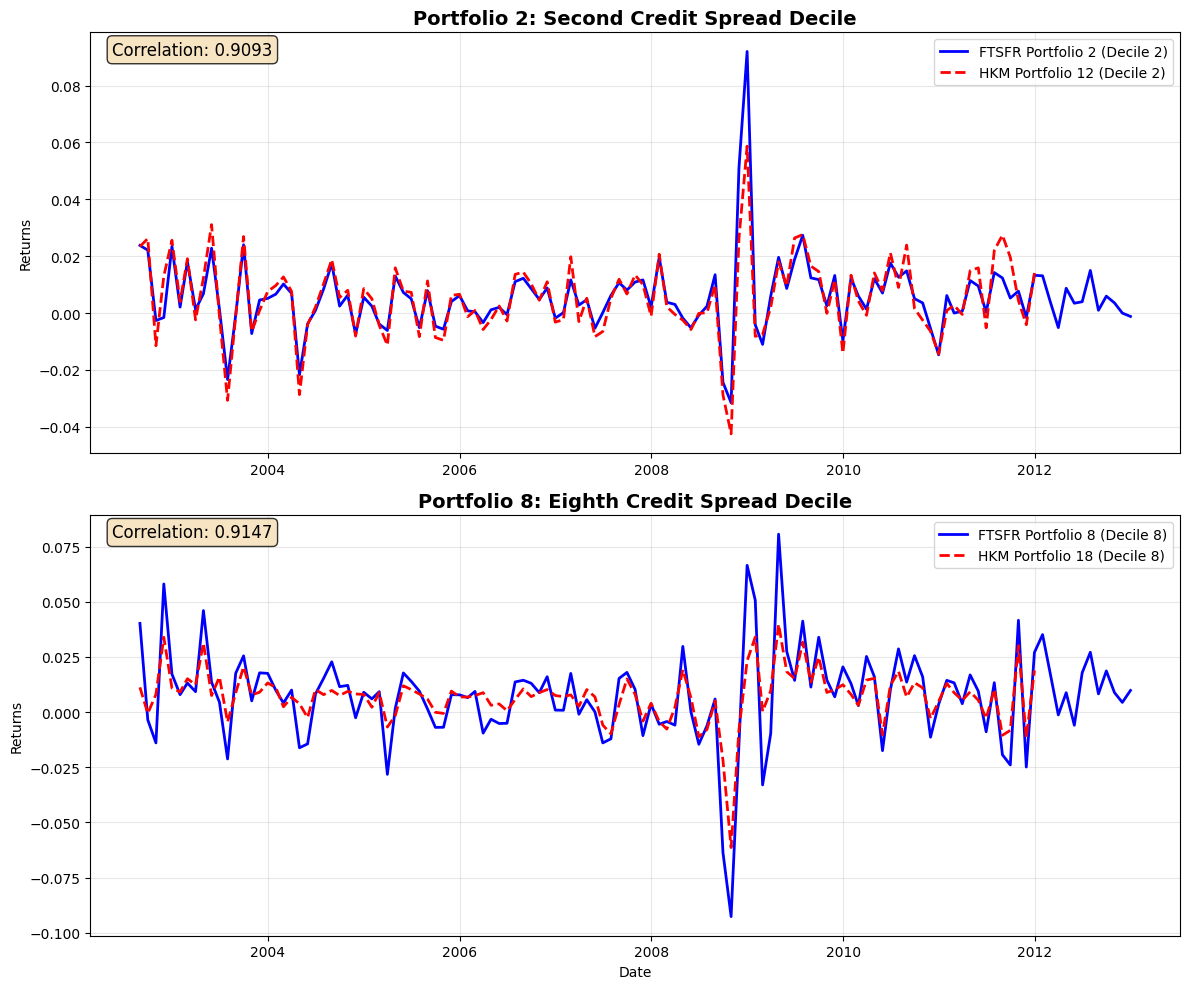
\includegraphics[width=0.8\textwidth]{../docs_src/corporate_returns_compare.png}
    \caption{Comparison of He, Kelly, and Manela (2017) corporate bond returns dataset with FTSFR dataset}
    \label{fig:corp_bond_returns_comparison}
  \end{figure}

\subsubsection{Sovereign Bonds}
\label{sec:sovereign}
% Borri and Verdelhan (2012) portfolios

\subsubsection{Options}
\label{sec:options}
% Constantinides, Jackwerth and Savov (2013) S&P 500 portfolios

Our monthly SPX options portfolio returns series follows the data cleaning and portfolio construction methodology of \citet{Constantinides2013} (``CJS''), which has become the canonical approach for constructing option-based portfolios. This framework forms the foundation for numerous studies in derivatives pricing and risk management. \citet{He2017} (``HKM'') later adapted the CJS methodology to create a set of 18 option portfolios from the 54 portfolios in CJS. Our dataset includes both the original 54 CJS portfolios and the 18 HKM portfolios, for a total of 72 unique SPX option portfolios.

The original CJS paper used data from 1986 through 2012 (26 years of data). As of the time of writing, due to the unavailability of SPX option data from 1985 to 1995, we replicated the \textbf{54 CJS portfolios} using data from \textbf{January 1996 to December 2019 (23 years of data)}. As shown in Figure~\ref{fig:spx_options_over_time}, the number of SPX option observations has increased significantly over time, and since the volume of SPX options traded prior to 1996 was very low, we believe that our dataset from 1996 to 2019, while 3 years shorter is far richer in content and more relevant for current and future research.

The process to construct our returns series involved two major phases: (1) Replicating with the highest practical fidelity the raw daily data filtration and monthly portfolio construction procedures outlined in \citet{Constantinides2013}, and (2) Transforming these returns series into the 18 portfolios outlined in \citet{He2017}.

\paragraph{Options Data Series Access}

The final FTFSR data series comprise the monthly leverage-adjusted returns for call and put portfolios for both CJS 2013 (54 portfolios) and HKM 2017 (18 portfolios) for the period from Jan 1996--Dec 2019. Each portfolio is identified by a unique string of the form: 

\begin{center}
{\texttt{\{option type 'C' or 'P'\}\_\{moneyness $\times$ 1000\}\_\{maturity in days\}}}
\end{center}

Where ``C'' indicates a call option portfolio, ``P'' indicates a put option portfolio, ``moneyness'' is the strike price divided by the index price (e.g. 0.95, 1.00, 1.05), and ``maturity in days'' is the number of days to expiration (e.g. 30, 60, 90, 120, 150, 180). For example, the portfolio string ``C\_950\_30'' indicates a call option portfolio with moneyness of 0.95 and maturity of 30 days.



\paragraph{Phase 1a: Data Filtration in \citet{Constantinides2013}}

In order to minimize possible quoting errors, CJS filtered the raw options data through three levels of filters. The filters are applied to the trade-in (buy) side to ensure the portfolios are buying into reliable quotes. When positions are exited, if there is no quote in the filtered data, the raw data is searched. These filters are detailed in \textit{Appendix B} of CJS.




\paragraph{\textit{Level 1 Filters}}
\begin{itemize}
  \item \textbf{Identical Filter:} Retain only one instance of quotes with the same \textit{option type}, \textit{strike price}, \textit{expiration date/maturity}, and \textit{price}.
  \item \textbf{Identical Except Price Filter:} For sets of quotes with identical terms (\textit{type}, \textit{strike}, and \textit{maturity}) but different prices, keep the quote whose \textit{T-bill-based implied volatility} is closest to that of its \textit{moneyness neighbors}, and delete the others.
  \item \textbf{Bid = 0 Filter:} Drop quotes with a \textit{bid price} of zero, thereby avoiding low-valued options. Also, a zero bid may indicate censoring as negative bids cannot be recorded.
  \item \textbf{Volume = 0 Filter:} Drop quotes with zero volume. Appendix B of CJS does not explicitly detail this filter, but we list it here for completeness since it is included in Table B.1 (Filters) of CJS. However, given that \textit{Appendix B} of \citet{Constantinides2013} did not describe this filter, we assume its inclusion in Table B.1 (Filter) of CJS was an error, and we have not implemented this filter in our replication.
\end{itemize}


\paragraph{\textit{Level 2 Filters}}
\begin{itemize}
  \item \textbf{Days to Maturity Filter:} Drop options with fewer than seven or more than 180 calendar days to expiration.
  \item \textbf{Implied Volatility Filter:} Remove all option quotes with implied volatilities lower than 5\% or higher than 100\%, computed using T-bill interest rates.
  \item \textbf{Moneyness Filter:} Remove all option quotes with moneyness (the ratio of strike price to index price) below 0.8 or above 1.2. These options have little value beyond their intrinsic value and are also very thinly traded.
  \item \textbf{Implied Interest Rate Filter:} Compute implied volatilities using T-bill interest rates from the Federal Reserve’s H.15 release, assigning the closest available rate to each observation. Since T-bill rates may not be relevant for short maturities, we also compute a put-call parity-implied interest rate by imposing put-call parity on put-call pairs and adjusting the interest rate. We remove pairs with negative implied interest rates and assign the median-implied rate to all quotes of the same maturity and moneyness between 0.95 and 1.05, interpolating as needed.
  \item \textbf{Unable to Compute IV Filter:} Remove quotes that imply negative time value.
\end{itemize}

\paragraph{\textit{Level 3 Filters}}
\begin{itemize}
  \item \textbf{IV Filter:} The IV filter removes volatility outliers to reduce the prevalence of apparent butterfly arbitrage. This involves dropping calls and puts that have the same expiration date and strike price, but have anomalous prices due to extreme implied volatility values. For each date and maturity, we fit a quadratic curve to the implied volatility of puts and calls (separately) through the observed log implied volatilities.
  \item \textbf{Put-Call Parity Filter:} The puts and calls need to be matched up based on trading date, expiry date, and option type. We then calculate the put-call parity implied interest rate, and filter out outliers based on the standard deviation of the relative distance between the interest rate implied by put-call parity, and the calculated daily median 3-month T-bill rate from the pulled data.
\end{itemize}


\begin{figure}[H]
  \centering
  \begin{tabular}{@{}c@{}}
    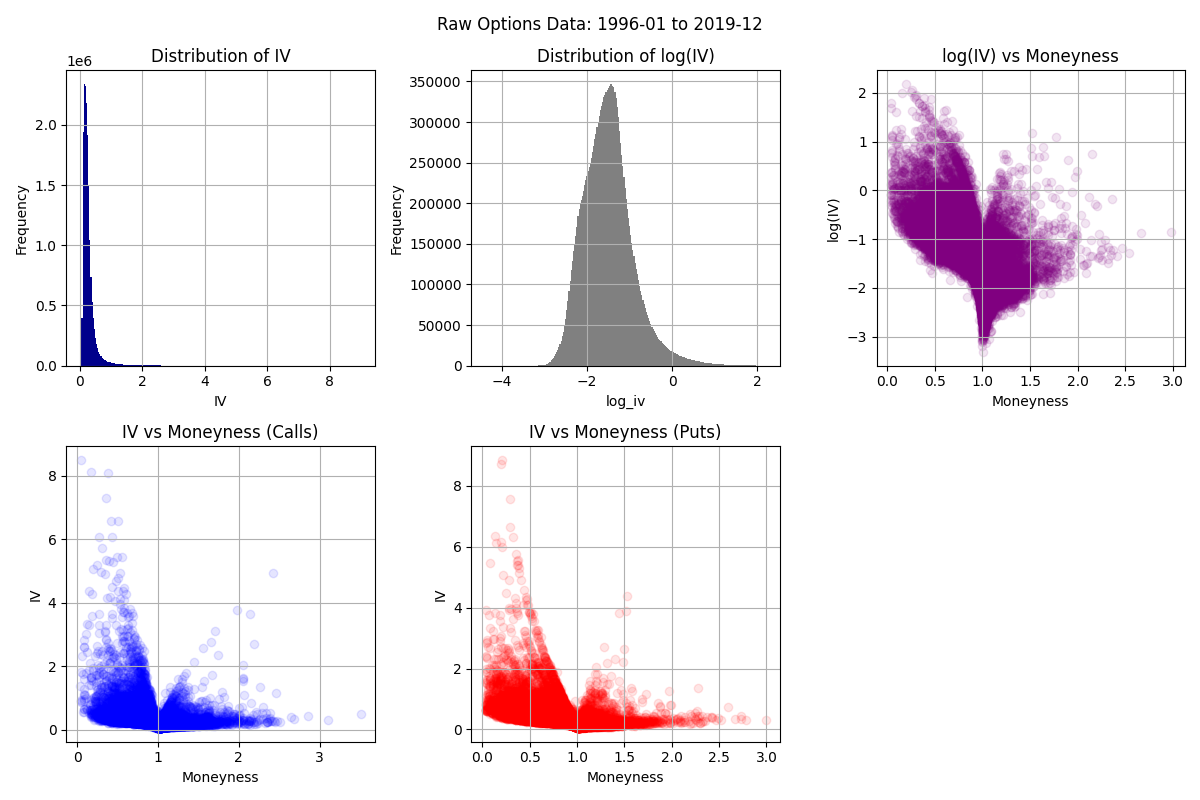
\includegraphics[width=\linewidth,height=0.666\linewidth]{../docs_src/RAW_1996-01_2019-12_iv.png}
  \end{tabular}
  \caption{Some visualizations of the raw SPX options data, prior to application of any filters. Each dot / point on these charts represents a single option in the raw data. Note that the time dimension is not shown, so this is a cross-sectional view of all options in the dataset.}
  \label{fig:raw_spx_options_data}
\end{figure}

\begin{figure}[H]
  \centering
  \begin{tabular}{@{}c@{}}
    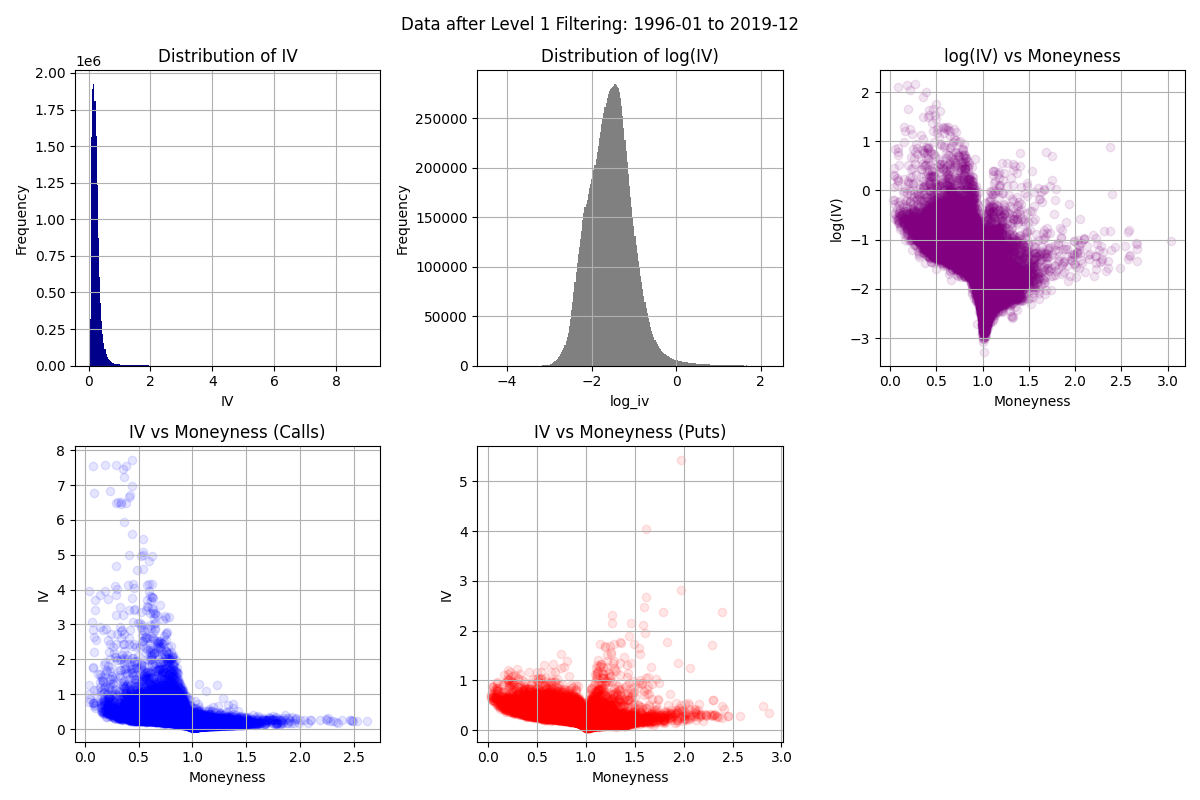
\includegraphics[width=\linewidth,height=0.666\linewidth]{../docs_src/L1_1996-01_2019-12_iv.png}
  \end{tabular}
  \caption{SPX options remaining after application of Level 1 filters. Notice reduction in outliers and cleaner distribution of volatility vs moneyness.}
  \label{fig:l1_spx_options_data}
\end{figure}


\begin{figure}[H]
  \centering
  \begin{tabular}{@{}c@{}}
    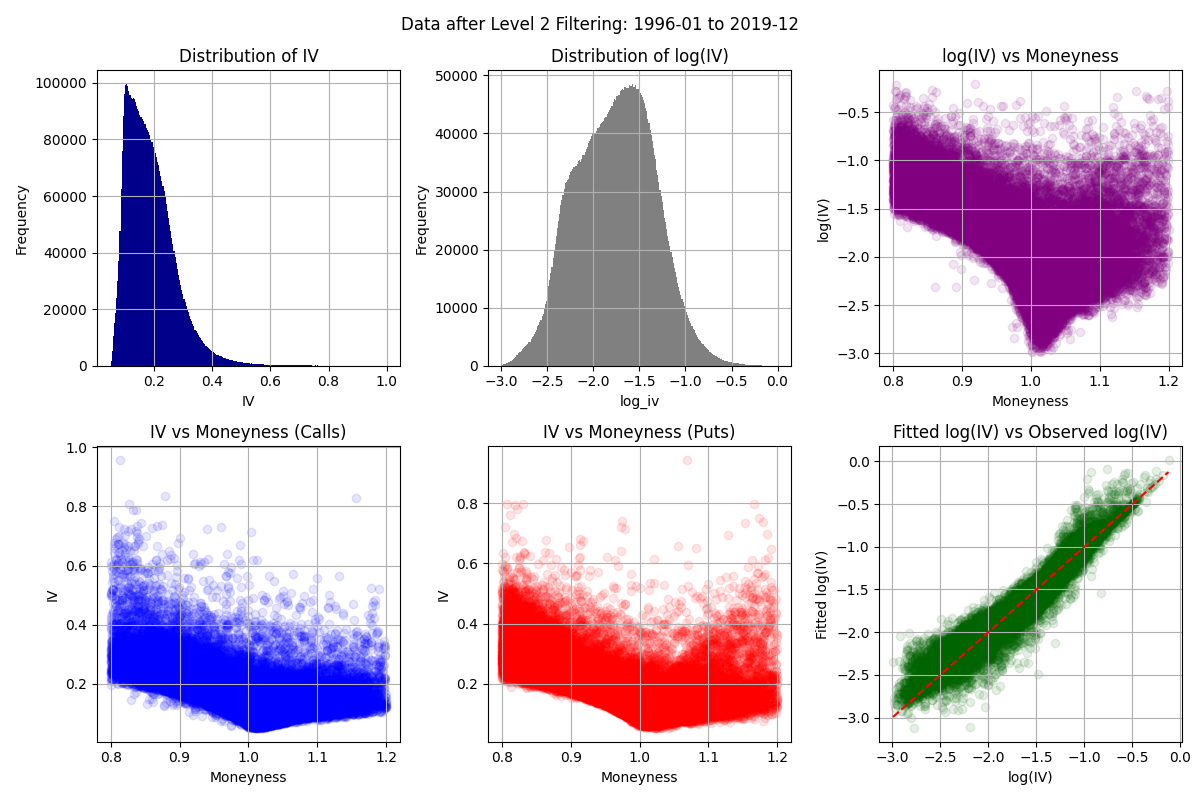
\includegraphics[width=\linewidth,height=0.666\linewidth]{../docs_src/L2_1996-01_2019-12_iv.png}
  \end{tabular}
  \caption{SPX options remaining after Level 2 filters.}
  \label{fig:l2_spx_options_data}
\end{figure}


\begin{figure}[H]
  \centering
  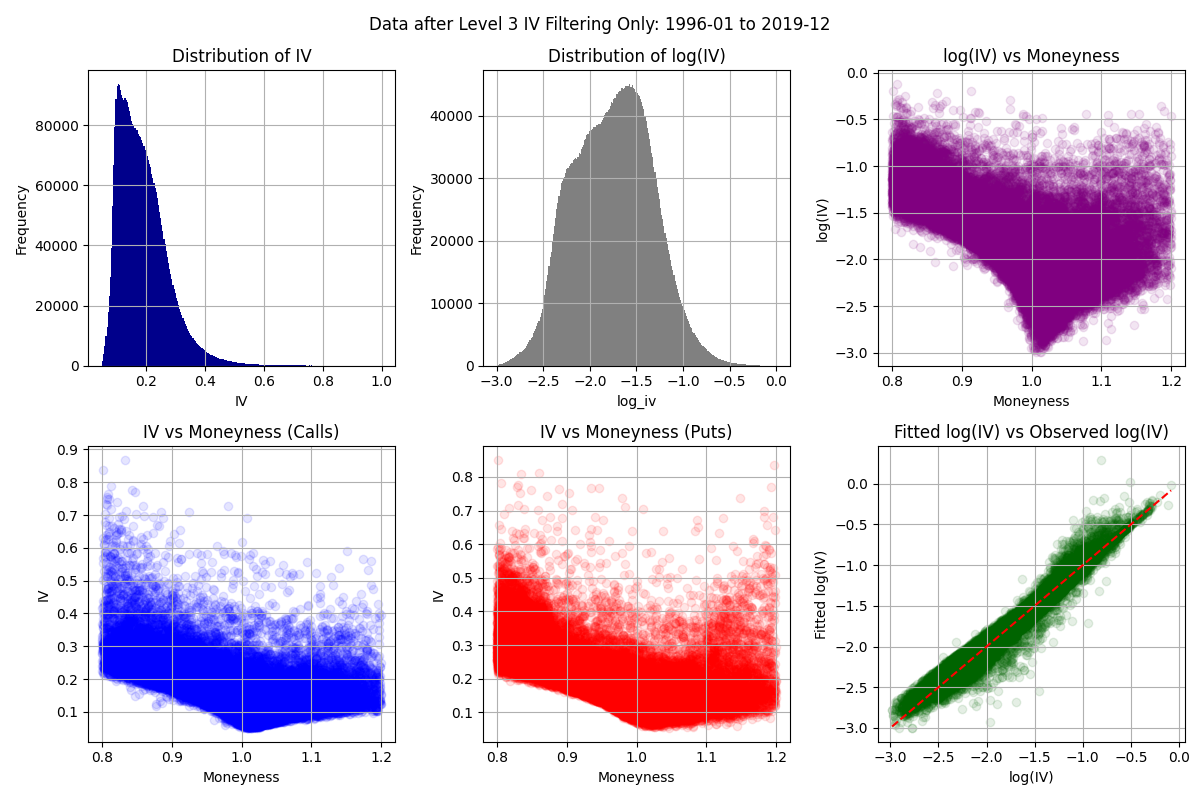
\includegraphics[width=\linewidth,height=0.666\linewidth]{../docs_src/L3_IV_1996-01_2019-12_iv.png}
  \caption{SPX options remaining after the Level 3 Implied Volatility filter (only).}
  \label{fig:l3_iv_only_spx_options_data}
\end{figure}


\begin{figure}[H]
  \centering
  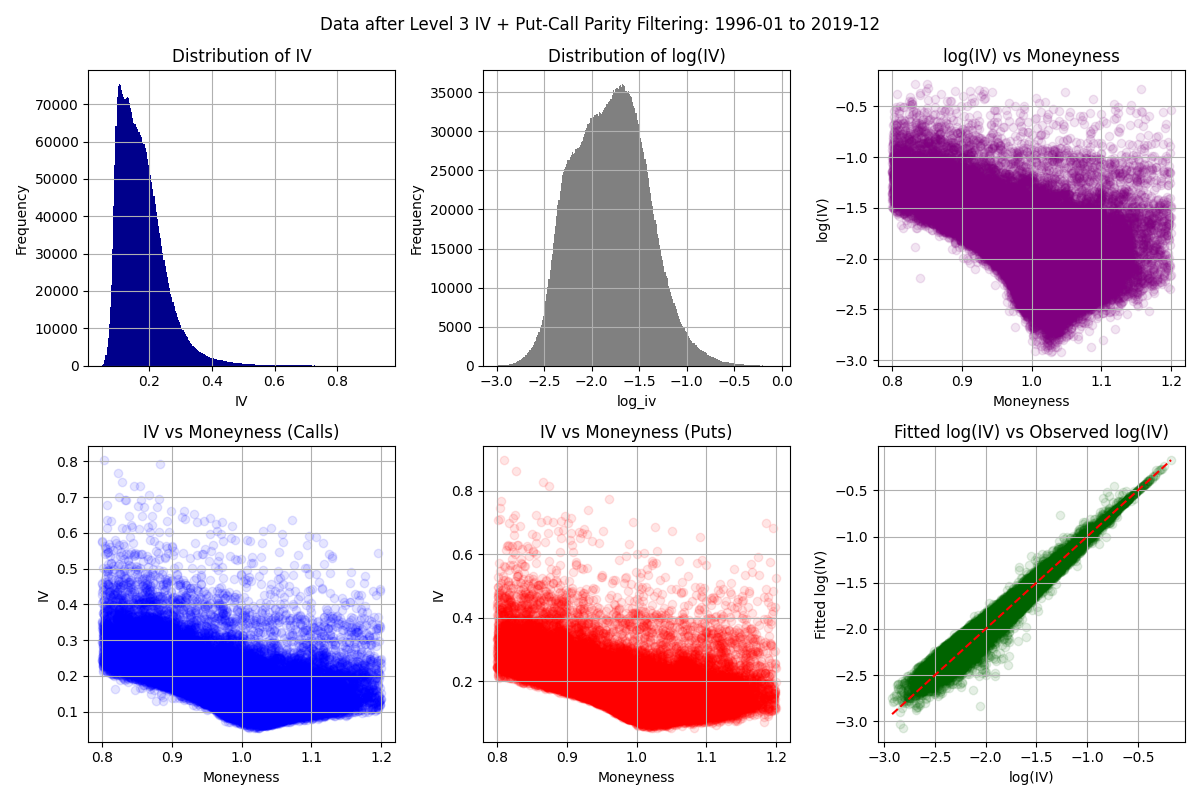
\includegraphics[width=\linewidth,height=0.666\linewidth]{../docs_src/L3_IV_PCP_1996-01_2019-12_iv.png}
  \caption{SPX options remaining after the Level 3 Implied Volatility and Put-Call Parity filters. Note how we observe the emergence of a volatility smile after the application of these filters.}
  \label{fig:l3_iv_pcp_spx_options_data}
\end{figure}


\paragraph{\textit{Phase 1b: Portfolio Construction in \citet{Constantinides2013}}}
\subsubsection*{Construction of Monthly Leverage-Adjusted Portfolio Returns in CJS}

\paragraph{Process}
The construction of the 27 call and 27 put portfolios in CJS is a multi-step process, with the objective of developing portfolio returns series that are stationary and only moderately skewed. The discrete bucketing of moneyness and days to maturity leads to multiple candidate options for each portfolio on each trading day. These options are given weights according to a \textbf{bivariate Gaussian weighting kernel} in moneyness and maturity (bandwidths: 0.0125 in moneyness and 10 days to maturity).

Each portfolio's daily returns are initially calculated as simple arithmetic returns, assuming the option is bought and sold at its bid-ask midpoint at each rebalancing. The one-day arithmetic return is then converted to a \textbf{leverage-adjusted return}. This procedure is achieved by calculating the one-day return of a hypothetical portfolio with $\omega_{BSM}^{-1}$ dollars invested in the option, and $(1 - \omega_{BSM}^{-1})$ dollars invested in the risk-free rate, where $\omega_{BSM}$ is the Black-Scholes-Merton elasticity based on the implied volatility of the option.

\begin{align}
\omega_{\text{BSM, Call}} &= \frac{\partial C_{\text{BSM}}}{\partial S} \cdot \frac{S}{C_{\text{BSM}}} > 1 \\
\omega_{\text{BSM, Put}}  &= \frac{\partial P_{\text{BSM}}}{\partial S} \cdot \frac{S}{P_{\text{BSM}}} < -1
\end{align}

Each \textbf{leverage-adjusted call portfolio} comprises a long position in a fraction of a call, and some investment in the risk-free rate.

Each \textbf{leverage-adjusted put portfolio} comprises a short position in a fraction of a put, and more than 100\% investment in the risk-free rate.

\textcolor{blue}{
Below, we formalize the CJS portfolio construction process for a single trading day $t$ and a set of candidate call or put options. Each portfolio is defined by \textbf{option type} (call or put), \textbf{target moneyness} (specifically $0.90$, $0.925$, $0.95$, $0.975$, $1.00$, $1.025$, $1.05$, $1.075$, $1.10$), and \textbf{target maturity} (specifically $30$, $60$, or $90$ days). On any given day, available options rarely match the targets exactly; instead, multiple candidate options may be close in moneyness and maturity. Each candidate option has its own price and sensitivity to the underlying index. \\ To aggregate these candidates, CJS applies a \textbf{Gaussian kernel in moneyness and maturity}, assigning weights to each option based on proximity to the targets. The \textbf{kernel-weighted average price} is used as the portfolio's option component. Portfolio returns are \textbf{leverage-adjusted using Black-Scholes-Merton elasticity} to standardize sensitivity across moneyness levels. \\ The \textbf{daily portfolio return} from $t$ to $t+1$ is computed as the kernel-weighted average return of the candidate options, using weights from day $t$. This approach ensures that each portfolio reflects the closest available options to the target characteristics, with appropriate adjustment for \textbf{leverage} and \textbf{sensitivity}.}

\subsubsection*{1. Gaussian Kernel Weighting}

Let:
\begin{itemize}
  \item $m_{i}$ = moneyness of option $i$
  \item $\tau_{i}$ = days to maturity of option $i$
  \item $k_{s}$ = target moneyness
  \item $\tau$ = target maturity
  \item $h_{m}$, $h_{\tau}$ = bandwidths for moneyness and maturity
  \item $d_{i}^2 = \left( \frac{m_{i} - k_{s}}{h_{m}} \right)^2 + \left( \frac{\tau_{i} - \tau}{h_{\tau}} \right)^2$
\end{itemize}

Then the unnormalized Gaussian weight for option $i$ is:
\[
w_{i}^* = \exp\left( -\frac{1}{2} d_{i}^2 \right)
\]

The normalized kernel weight:
\[
w_{i} = \frac{w_{i}^*}{\sum_j w_j^*}
\]

\subsubsection*{2. Option Elasticity}

Let:
\begin{itemize}
  \item $S_{t}$ = underlying index level at time $t$
  \item $P_{i}$ = price of option $i$
  \item $\Delta_{i}$ = option delta
\end{itemize}

Then:
\[
\varepsilon_{i} = \frac{S_t \cdot \Delta_{i}}{P_{i}}
\]

\subsubsection*{3. Arithmetic Return of Option $i$}

Let:
\begin{itemize}
  \item $P_{i,t-1}$ = price of option $i$ at time $t-1$
  \item $P_{i,t}$ = price of option $i$ at time $t$
\end{itemize}

Then:
\[
r_{i} = \frac{P_{i,t} - P_{i,t-1}}{P_{i,t-1}}
\]

\subsubsection*{4. Leverage-Adjusted Portfolio Construction}

Let:
\begin{itemize}
  \item $r_{f}$ = risk-free rate on day $t$
\end{itemize}

The leverage-adjusted return of the call portfolio is:
\[
R_t^{call} = \sum_{i} w_{i} \cdot \frac{1}{\varepsilon_{i}} \cdot r_{i} + \left(1 - \sum_{i} w_{i} \cdot \frac{1}{\varepsilon_{i}} \right) \cdot r_f
\]

The leverage-adjusted return of the put portfolio is:
\[
R_t^{put} = -\sum_{i} w_{i} \cdot \frac{1}{\varepsilon_{i}} \cdot r_{i} + \left(1 + \sum_{i} w_{i} \cdot \frac{1}{\varepsilon_{i}} \right) \cdot r_f
\]



\subsubsection*{5. Handling Missing Data (NaN Filling)}

CJS implement a multi-step process to address options with missing prices, as detailed in Section 1.3 ``Portfolio Formation'' of their paper. We reserve the implementation of this NaN-filling procedure for a future version of this dataset. For the current version, we compound the daily portfolio returns into monthly returns, which matches the final form of the data utilized in the paper.


\paragraph{\textit{Phase 2: Returns Series Transformation in \citet{He2017}}}
\subsubsection*{Construction of 18 Portfolio Return Series in HKM}

\citet{He2017} reduce the 54 portfolios constructed in \citet{Constantinides2013} to 18 portfolios by taking an equal-weight average across the three maturities (30, 60, 90 days) for all CJS portfolios with the same moneyness. We implement that procedure to obtain the final return series for the FTSFR.

Let \( R_{m,j,t} \) be the return for moneyness \( m \), maturity \( j \), at time \( t \).
The HKM portfolio return for moneyness \( m \) at time \( t \) is:
\[
R_{m,t}^{\mathrm{HKM}} = \frac{1}{3} \sum_{j=1}^{3} R_{m,j,t}
\]
For each moneyness group, the HKM portfolio return is the simple average of the three corresponding CJS portfolio returns (one for each maturity) at each time point.

This averaging is done separately for calls and puts, resulting in 9 call portfolios and 9 put portfolios (total 18 portfolios).



\subsubsection*{Portfolio Returns Analysis}

The objective of the data filtration process was to construct portfolios whose returns are approximately normal and only moderately skewed. We analyzed the distributional properties of the 54 CJS portfolios and the 18 HKM portfolios using standard statistical tests and summary statistics.

\paragraph{Statistical Normality Tests}
To assess the normality of portfolio returns, we applied several standard tests:
\begin{itemize}
  \item \textbf{Shapiro-Wilk Test:} Tests the null hypothesis that the data are drawn from a normal distribution. The test statistic is
  \[
  W = \frac{\left( \sum_{i=1}^n a_i x_{(i)} \right)^2}{\sum_{i=1}^n (x_i - \bar{x})^2}
  \]
  where $x_{(i)}$ are ordered sample values and $a_i$ are constants.
  \item \textbf{Jarque-Bera Test:} Tests whether sample skewness and kurtosis match a normal distribution. The test statistic is
  \[
  JB = \frac{n}{6} \left( S^2 + \frac{(K-3)^2}{4} \right)
  \]
  where $S$ is sample skewness and $K$ is sample kurtosis.
  \item \textbf{D'Agostino and Pearson's Normality Test (Normaltest):} Combines skewness and kurtosis to test for normality.
\end{itemize}
Low $p$-values (typically $<0.05$) indicate rejection of normality.

\paragraph{Summary Statistics}
Table~\ref{tab:portfolio_stats} presents descriptive statistics for the returns of the CJS and HKM portfolios. The statistics include count, mean, standard deviation, minimum, 25th percentile, median, 75th percentile, and maximum, following the convention of \texttt{pd.DataFrame.describe()}.

\begin{table}[H]
  \centering
  \caption{Descriptive Statistics of Portfolio Returns}
  \label{tab:portfolio_stats}
  \begin{tabular}{lcc}
    \toprule
    \textbf{Statistic} & \textbf{CJS Portfolios} & \textbf{HKM Portfolios} \\
    \midrule
    Count   & 54                          & 18                          \\
    Mean    & 1.64 (skew), 14.5 (kurtosis)  & 1.87 (skew), 16.8 (kurtosis) \\
    Std     & 2.26 (skew), 23.8 (kurtosis)  & 2.64 (skew), 30.3 (kurtosis) \\
    Min     & -0.91 (skew), 0.7 (kurtosis)  & -0.91 (skew), 0.7 (kurtosis) \\
    25\%    & 0.12 (skew), 2.1 (kurtosis)   & 0.12 (skew), 2.1 (kurtosis) \\
    \rowcolor{blue!20}
    Median  & 0.77 (skew), 4.6 (kurtosis)   & 0.78 (skew), 3.1 (kurtosis) \\
    75\%    & 2.41 (skew), 12.3 (kurtosis)  & 2.41 (skew), 12.3 (kurtosis) \\
    Max     & 11.1 (skew), 152.7 (kurtosis) & 9.8 (skew), 129.3 (kurtosis) \\
    \bottomrule
  \end{tabular}
\end{table}

\textbf{Note:} We did not implement the NaN-filling logic described in the original CJS paper. As a result, missing data may affect the distributional properties of the portfolio returns, and these results and conclusions may change in future versions once NaN handling is incorporated.

\paragraph{Results for CJS Portfolios}

Nearly all CJS portfolios reject normality based on the Shapiro-Wilk, Jarque-Bera, and Normaltest $p$-values, which are close to zero. The mean skewness is 1.64 and the median is 0.77, indicating distributions are generally right-skewed with long right tails. The mean kurtosis is 14.5 and the median is 4.6, suggesting many portfolios are leptokurtic (fat-tailed), with some experiencing rare but large return shocks. However, the median skewness and kurtosis are much closer to the normal values (skewness $=0$, kurtosis $=3$), implying that most portfolios are only moderately skewed and not excessively heavy-tailed. These results confirm that the filtration and leverage-adjustment procedures substantially mitigate extreme non-normality, achieving the authors' objective of constructing portfolios with returns that are approximately normal and only moderately skewed.

\paragraph{Results for HKM Portfolios}
Most HKM portfolios also reject normality, although a few have higher $p$-values and may plausibly be normal. The mean skewness is 1.87 and the median is 0.78, again showing generally positive skewness. The mean kurtosis is 16.8 and the median is 3.1, which is very close to the normal value of 3. This suggests that, while some portfolios have extreme outliers, the median HKM portfolio is only moderately skewed and has kurtosis similar to a normal distribution. These findings further validate that the aggregation and transformation steps in HKM produce portfolio returns with moderate skewness and near-normal kurtosis.

\paragraph{Overall Findings}
In summary, the data filtration and portfolio construction procedures yield return series that are not perfectly normal, but the median portfolio for both CJS and HKM is much closer to normal and only moderately skewed. This demonstrates that the authors' objectives were largely met: the median portfolio is well-suited for empirical asset pricing tests that assume approximate normality, even though some portfolios remain highly non-normal due to outliers. The successful replication of these distributional properties confirms the effectiveness of the canonical cleaning and construction methods.



\subsubsection{Foreign Exchange}
\label{sec:fx}
% Lettau et al. (2014) and Menkhoff et al. (2012)
The Foreign Currencies returns series we generated uses spot rate changes and local repo rates to generate a USD-based
foreign currency returns. 

We are replicating a process where we convert our USD into the foreign currency $i$ at end of day $t - 1$, 
invest it in the repo market, then switch the currency back to USD on day $t$. 

\begin{equation}
  ret_{t, i} \;=\; \frac{spot_{t - 1, i}}{spot_{t, i}} \times fret_{t, i}
\end{equation}

where
\begin{itemize}
 \item $i$ is the foreign currency
 \item $t$ is the date of the implied foreign currency return
 \item $ret$ is the return of USD invested in the foreign currency
 \item $fret$ is the return of the foreign currency when invested in their overnight repo market
 \item $spot$ is the spot price of the currency (how much 1 USD is worth in the foreign currency)
\end{itemize}

\begin{figure}
  \centering
  \begin{tabular}{@{}c@{}}
    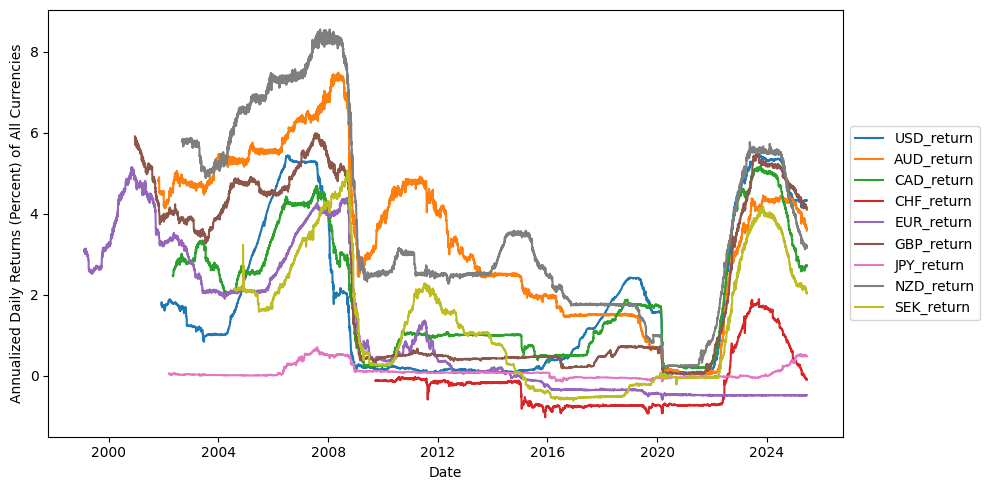
\includegraphics[width=.7\linewidth,height=200pt,width=400pt]{../docs_src/FX_returns.png} \\[\abovecaptionskip]
  \end{tabular}

  \caption{Foreign Currency Returns}
  \label{fig:fx_returns}
\end{figure}

\FloatBarrier

\subsubsection{Commodities}
\label{sec:commodities}
% Yang (2013) methodology

\subsubsection{Credit Default Swaps}
\label{sec:cds}
% Markit data following Palhares (2013)

[Asset class content to be filled in...]

\subsection{Arbitrage Spread Datasets}
\label{sec:arbitrage}

% TODO: Document each arbitrage spread construction
% For EACH arbitrage spread:
% - Explain the economic intuition behind the trade
% - Detail the exact construction methodology
% - Show replication of statistics from Siriwardane et al.
% - Discuss what violations of these spreads tell us about market segmentation

Following \cite{Siriwardane2021}, we construct various arbitrage spreads that measure market segmentation.

\subsubsection{Covered Interest Parity (CIP)}
% Construction using spot, forward FX and interest rates
     

During periods of market stress, such as the 2008 financial crisis and the 2020 COVID-19
pandemic, covered interest parity (CIP) may no longer hold as the forward---spot differential 
no longer exactly offsets interest‐rate differentials. Factors contributing to this phenomenon include:
Heightened Counterparty‐Credit Risk, Liquidity Constraints, or Regulatory Pressures.

In other periods, deviations from CIP typically stem from market inefficiencies and are 
small in magnitude and are short-lived in timeframe due to arbitrage activities.

Our analysis examines CIP deviations across eight G10 currencies against the USD, 
using data from 1999 onwards sourced through Bloomberg Terminal.

\paragraph{The dataset includes:}
\begin{itemize}
    \item Spot exchange rates for each currency pair
    \item 3-month forward points for each currency pair
    \item 3-month Overnight Index Swap (OIS) rates for each currency
\end{itemize}

\paragraph{Data Standardization:}
\begin{itemize}
    \item Forward points are scaled appropriately (per 10,000 for most currencies, per 100 for JPY)
    \item Currencies conventionally quoted as USD-per-foreign-currency (EUR, GBP, AUD, NZD) are converted to reciprocal rates for consistency
    \item OIS rates serve as our risk-free benchmark to align with other arbitrage spread studies
\end{itemize}

We successfully replicate the CIP spreads as calculated by Siriwardane et al. (2023),
as seen in this side by side comparison of our calculated currency respective
arbitrage spreads versus those reported in their paper.

\begin{figure}
  \centering
  \begin{tabular}{@{}c@{}}
    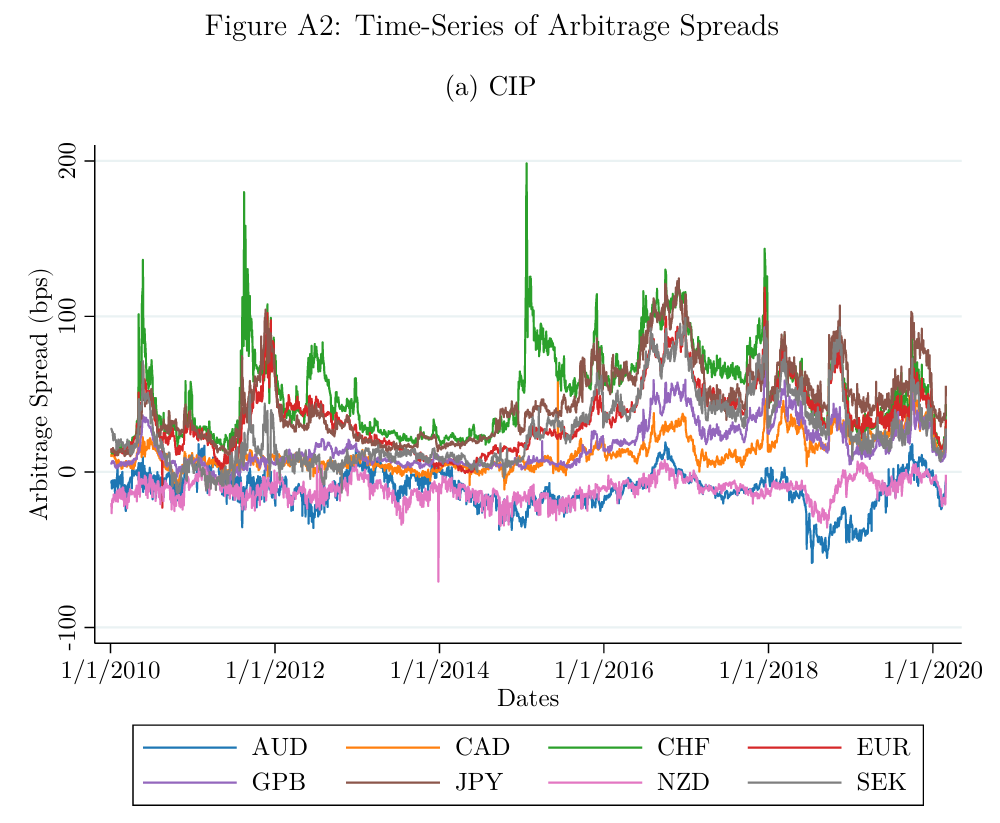
\includegraphics[width=.7\linewidth,height=210pt,width=350pt]{../docs_src/SegArb_CIP_Timeseries.png} \\[\abovecaptionskip]
    \small (a) Findings in Siriwardane et al. (2023)
  \end{tabular}

  \vspace{\floatsep}

  \begin{tabular}{@{}c@{}}
    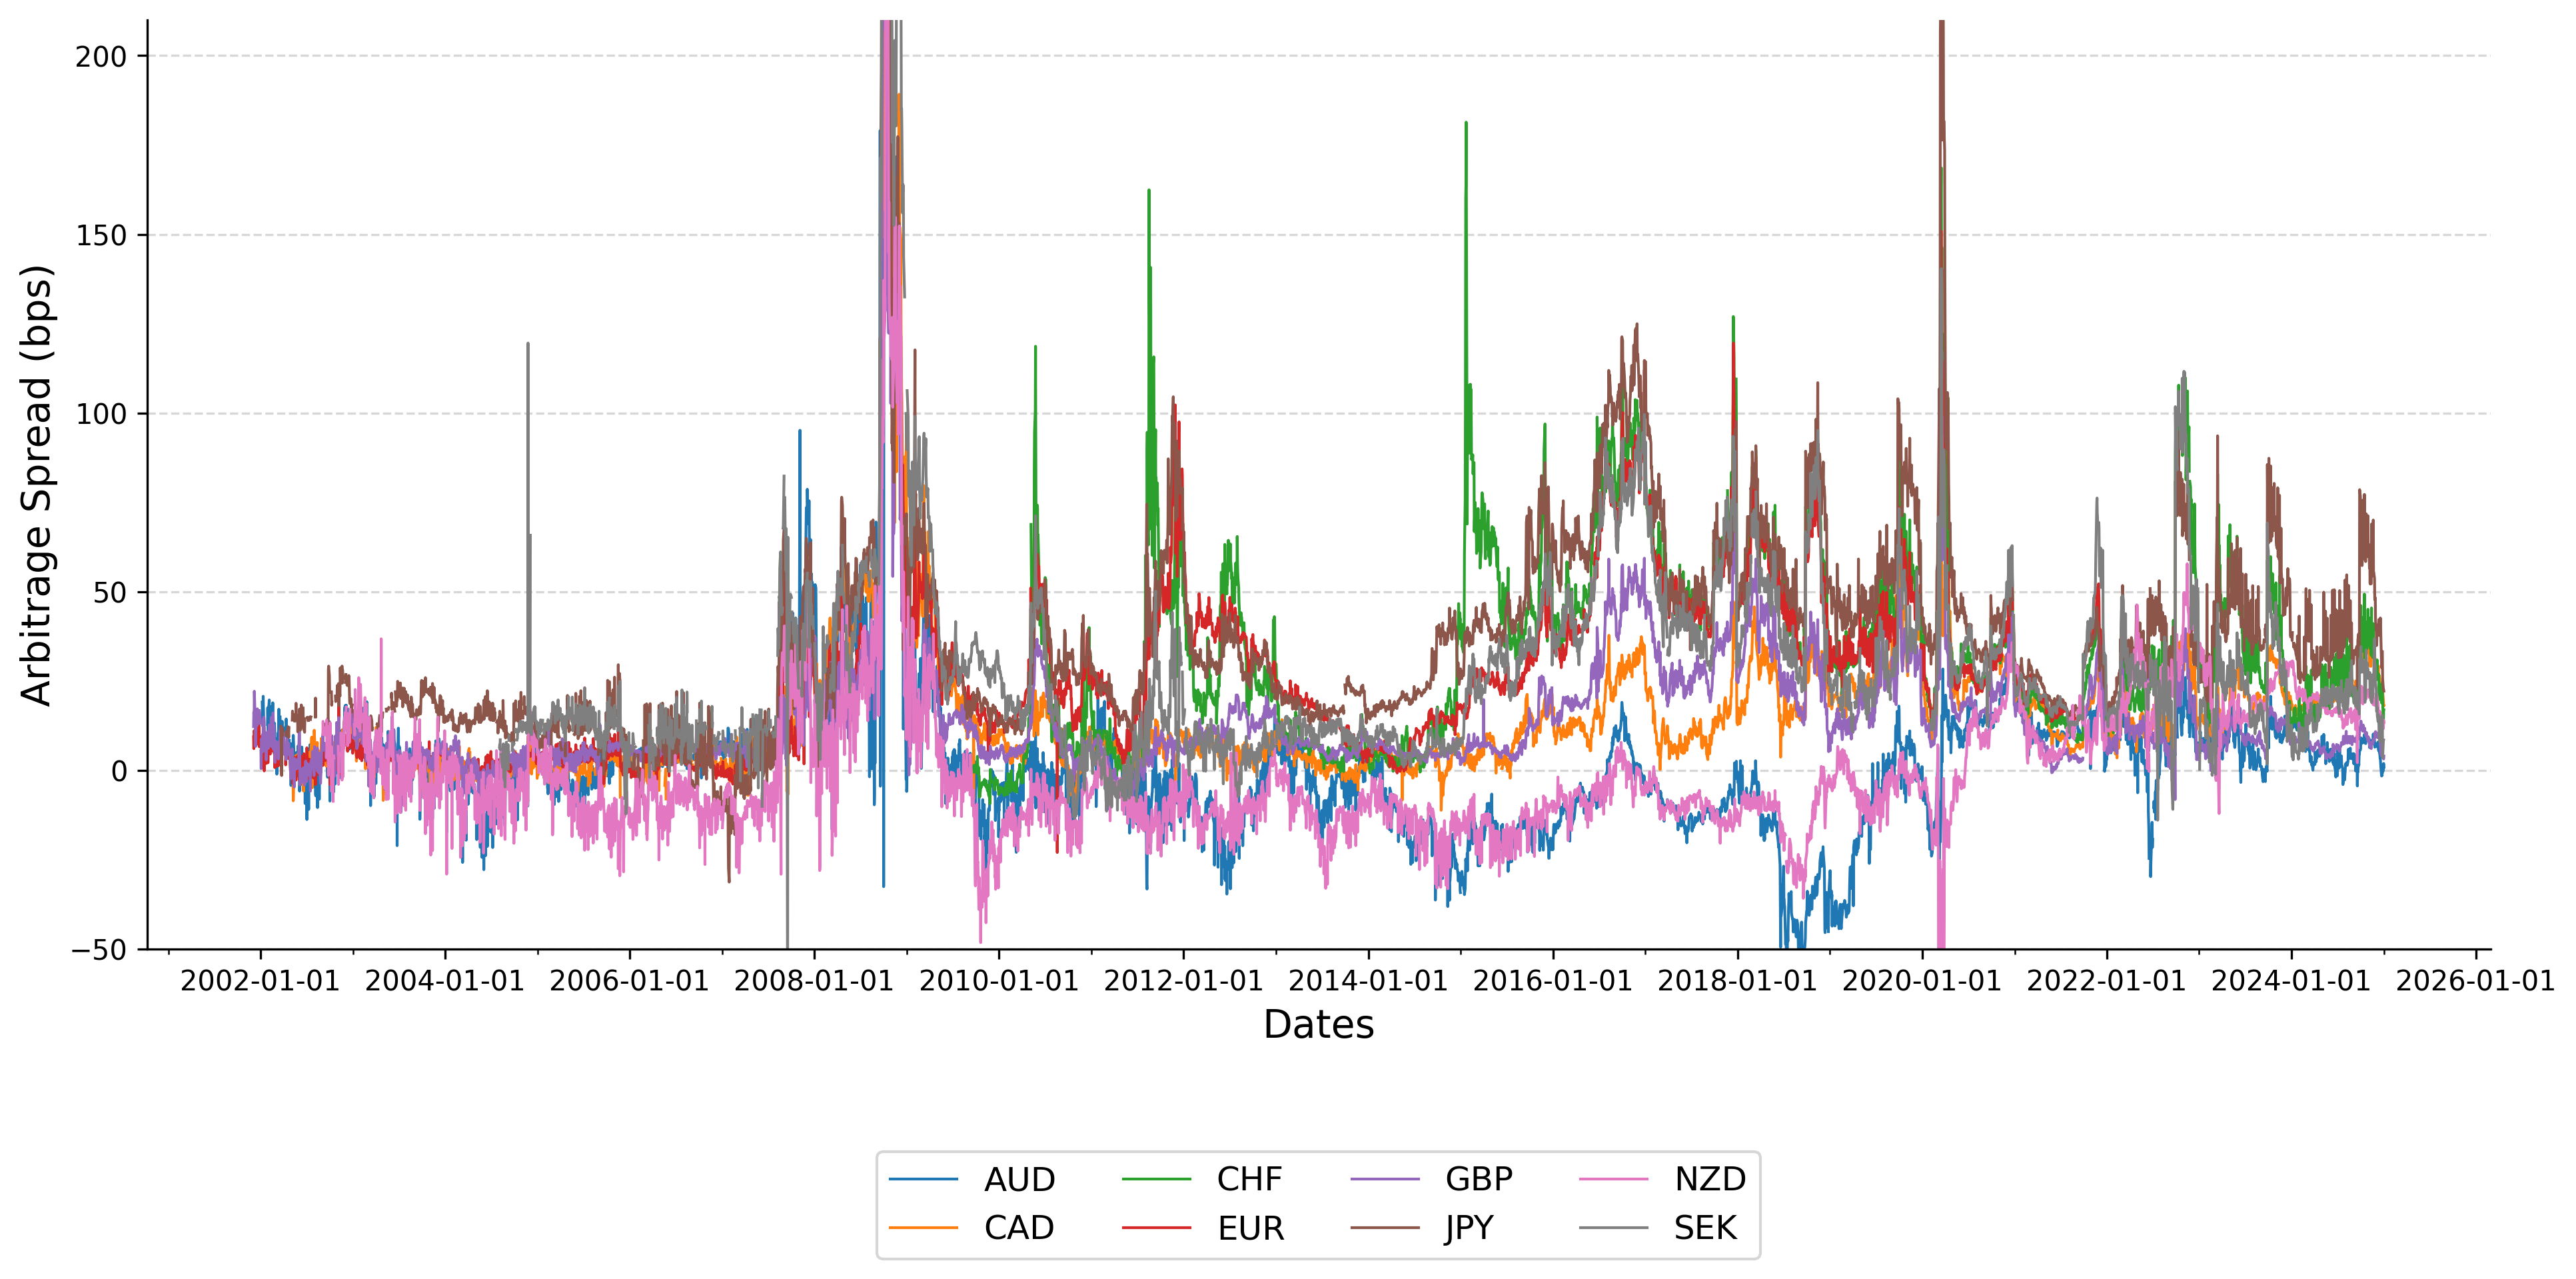
\includegraphics[width=.7\linewidth,height=200pt,width=400pt]{../docs_src/CIP_replicate.png} \\[\abovecaptionskip]
    \small (b) Our findings
  \end{tabular}

  \caption{Comparison of CIP Arbitrage spreads}
  \label{fig:cip_comparison}
\end{figure}

\FloatBarrier


During the overlapping periods of both datasets, the CIP spreads are nearly identical.
Our findings confirm the presence of CIP deviations, particularly during periods of
market stress, consistent with the conclusions drawn by Siriwardane et al. (2023).


\subsubsection{Box Spread Arbitrage}
% Options-based arbitrage using put-call parity

\subsubsection{Equity Spot-Futures Basis}
% Cash vs futures arbitrage

\subsubsection{Treasury Spot-Futures Basis}
% Government bond basis trades

\subsubsection{Treasury-Swap Spread}
% Treasury vs interest rate swap arbitrage

\subsubsection{TIPS-Treasury Spread}
% Inflation-linked vs nominal bond spreads

\subsubsection{CDS-Bond Basis}
% Credit default swap vs cash bond arbitrage

Credit Default Swaps (CDS) are "insurance contracts" against the default of underlying
corporate debt. The buyer of CDS protection pays a the CDS spread as a 
fixed annuity premium to the seller for a horizon $\tau$. If there is a default
before the time horizon $\tau$, the buyer receives the difference between
the bond's par value and its market value from the seller. 
As a result, the payoff of this portfolio should not deviate from the risk free bond. 
The resulting difference between CDS spread and floating rate spread (corporate bond rate - risk free rate)
is defined by the authors as the CDS-basis.

The authors define the CDS basis (CB) as

\begin{equation}
  CB_{i,t,\tau} \;=\; CDS_{i,t,\tau} \;-\; FR_{i,t,\tau},
\end{equation}

where:
\begin{itemize}
  \item $FR_{i,t,\tau}$ = time $t$ floating‐rate spread implied by a fixed‐rate corporate bond issued by firm $i$ at tenor $\tau$,
  \item $CDS_{i,t,\tau}$ = time $t$ Credit Default Swap (CDS) par spread for firm $i$ with tenor $\tau$.
\end{itemize}

A negative basis implies an investor could earn a positive arbitrage profit by going long the bond and purchasing CDS protection. 
The investor would pay a lower par spread than the coupon of the bond itself and then receive value from the default.

The value of $FR$ is substituted by the paper with Z‐spread which we also modify in our construction. We address the substitution in detail later.

The value of CDS par spread is interpolated by the authors using a cubic spline function as
not all necessary tenors are present.

Given the CDS spread from above, traditional construction of a risk‐free rate for implied arbitrage implies the following return:

\begin{equation}
  rfr^{CDS}_{i,t,\tau} \;=\; y_{t,\tau} \;-\; CB_{i,t,\tau},
\end{equation}

where:
\begin{itemize}
  \item $y_{t,\tau}$ = maturity‐matched Treasury yield at time $t$.
\end{itemize}

The implied risk-free arbitrage is then defined as the treasury yield in addition to the basis received when executing the CDS basis trade (investor benefits from negative basis).

\subsubsection{Z-Spread (Zero-Volatility Spread)}

\paragraph*{Mathematical definition}
For a bond with cash-flows $CF_t$ at times $t=1,\dots,N$ and Treasury spot rates $s_t$,
\begin{equation*}
P = \sum_{t=1}^{N} \frac{CF_t}{\bigl(1+s_t+Z\bigr)^t}.
\end{equation*}
The constant $Z$ that solves this equation is the \textbf{Z-spread}.

\paragraph*{Intuition}
$Z$ is the uniform extra yield added to every point on the risk-free spot curve so that the discounted cash-flows equal the bond's dirty price $P$. It compensates investors for credit and liquidity risk relative to Treasuries.

\paragraph*{Link to Yield-to-Maturity}
Setting the Z-spread pricing equation equal to the standard YTM equation gives
\begin{equation}
\label{eq:ytm_z_spread}
\sum_{t=1}^{N}\frac{CF_t}{(1+y)^t}
=\sum_{t=1}^{N}\frac{CF_t}{\bigl(1+s_t+Z\bigr)^t}
\end{equation}
where $y$ is the bond's yield-to-maturity. Except for the trivial flat-curve case ($s_t=s$), equation (\ref{eq:ytm_z_spread}) has no algebraic solution—$y$ or $Z$ must be found numerically.

\paragraph*{Continuous-Compounding Identity}
Rewrite discounts as $e^{-r t}$. With PV-weights
\begin{equation*}
w_t=\frac{CF_t\,e^{-(s_t+Z)t}}{P},\qquad\sum_{t}w_t=1,
\end{equation*}
equation (\ref{eq:ytm_z_spread}) yields the convenient mean-value relationship
\begin{equation}
y \;=\; \sum_{t=1}^{N} w_t\,(s_t+Z)\tag{A2}
\end{equation}
Thus YTM is the PV-weighted average of the spot rates plus the Z-spread.

\paragraph*{Practical Proxy: YTM Credit Spread}
Analysts often approximate $Z$ with the \textbf{credit spread}
\begin{equation*}
\Delta y = y_{\text{bond}} - y_{\text{Treasury-DM}},
\end{equation*}
where $y_{\text{Treasury-DM}}$ is the yield on a Treasury portfolio matched to the bond's (modified) duration.

\paragraph*{Why it works}
\begin{enumerate}
    \item A small parallel shift $Z$ applied to all discount rates changes price by $-D_{\text{mod}}\;Z$. For modest spreads, this produces nearly the same price change as replacing the spot curve with a single rate shift $\Delta y$.
    \item Duration-matching the Treasury benchmark neutralises curve-shape effects, so $\Delta y$ isolates the average extra yield attributable to credit/liquidity risk.
    \item Empirically, $\Delta y$ tracks $Z$ closely for plain-vanilla, option-free bonds, making it a ``good-enough'' proxy when full spot-curve data or iterative Z-spread calculations are impractical.
\end{enumerate}

\paragraph*{Note}
Z-spread is said to be populated by Markit in the CDS dataset but during the reconstruction process we found no proxy. Thus, we chose our own construction.

\begin{figure}
  \centering
  \begin{tabular}{@{}c@{}}
    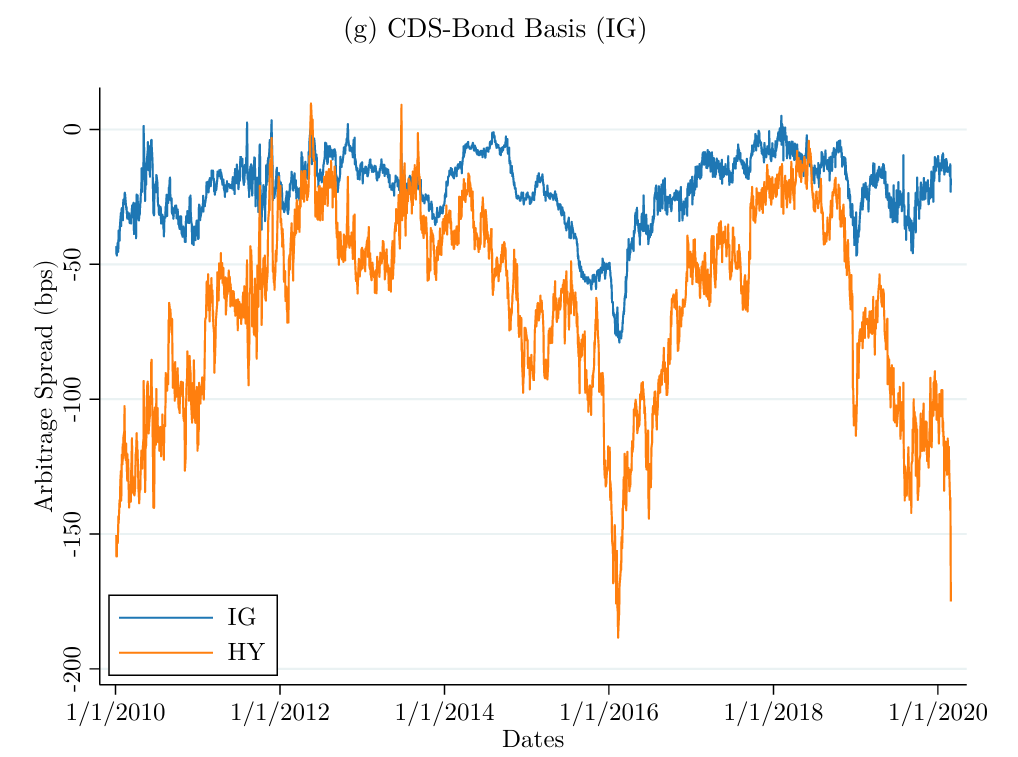
\includegraphics[width=.7\linewidth,height=210pt,width=350pt]{../docs_src/SegArb_CDS_Timeseries.png} \\[\abovecaptionskip]
    \small (a) Findings in Siriwardane et al. (2023)
  \end{tabular}

  \vspace{\floatsep}

  \begin{tabular}{@{}c@{}}
    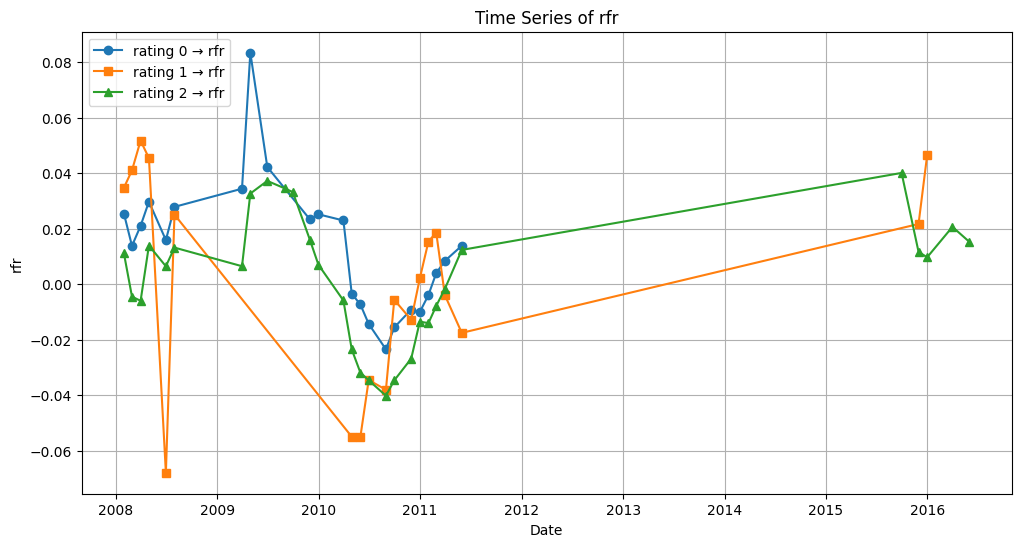
\includegraphics[width=.7\linewidth,height=200pt,width=400pt]{../docs_src/CDS_replicate.png} \\[\abovecaptionskip]
    \small (b) Our findings
  \end{tabular}

  \caption{Comparison of CDS Arbitrage spreads}
  \label{fig:CDS_replicate}
\end{figure}

\FloatBarrier

\subsection{Additional Financial Datasets}
\label{sec:additional_datasets}

% TODO: Document datasets for macroeconomic forecasting and financial stability monitoring

\subsubsection{Bank Call Report Data}
% NYU archive (Schnabl)

\subsubsection{Treasury Yield Curve}
% Fed data following Gürkaynak et al.

\subsubsection{Macroeconomic Indicators}
% FRED-MD and other macro series

\subsubsection{Bank-Specific Metrics}
% Using WRDS Bank Premium

[Additional datasets content to be filled in...]


\subsection{Additional Results}
\label{app:additional_results}
% Extended results tables and robustness checks

This section presents supplementary error metrics to provide a comprehensive view of model performance across all datasets. While the main text focuses on MASE and RMSE as primary metrics, we also report Symmetric Mean Absolute Percentage Error (sMAPE) and Mean Absolute Error (MAE) for completeness.

\subsubsection{Symmetric Mean Absolute Percentage Error (sMAPE)}

Table~\ref{tab:smape_results} presents sMAPE results across all model-dataset combinations. sMAPE provides percentage-based error measures that are symmetric and bounded, making them particularly useful for comparing performance across datasets with different scales and volatility patterns.

% sMAPE Results by Dataset and Model
% Generated automatically by create_results_tables2.py

\begin{table}[htbp]
\centering
\caption{sMAPE Results by Dataset and Model}
\label{tab:smape_results}
\scriptsize
\setlength{\tabcolsep}{2pt}
\renewcommand{\arraystretch}{0.85}
\begin{tabular}{@{}l@{\hspace{2pt}}@{\hspace{1pt}}r@{\hspace{1pt}}@{\hspace{1pt}}r@{\hspace{1pt}}@{\hspace{1pt}}r@{\hspace{1pt}}@{\hspace{1pt}}r@{\hspace{1pt}}@{\hspace{1pt}}r@{\hspace{1pt}}@{\hspace{1pt}}r@{\hspace{1pt}}@{\hspace{1pt}}r@{\hspace{1pt}}@{\hspace{1pt}}r@{\hspace{1pt}}@{\hspace{1pt}}r@{\hspace{1pt}}@{\hspace{1pt}}r@{\hspace{1pt}}@{\hspace{1pt}}r@{\hspace{1pt}}@{\hspace{1pt}}r@{\hspace{1pt}}@{\hspace{1pt}}r@{\hspace{1pt}}@{}}
\toprule
 & Naive & SN & Theta & ETS & ARIMA & DeepAR & NBEATS & NHITS & DLinear & NLinear & Transformer & TiDE & KAN \\
\midrule
\multicolumn{14}{l}{\textbf{Basis Spreads}} \\
CDS-Bond & 46.90 & 2.82 & 46.90 & 46.90 & 0.83 & 0.65 & 0.56 & 0.70 & 0.80 & 0.67 & 0.49 & \textbf{0.46} & 0.99 \\
CIP & \textbf{0.28} & 0.34 & \textbf{0.28} & \textbf{0.28} & 0.45 & 0.88 & 0.42 & 0.29 & 0.64 & 0.32 & 0.71 & 0.50 & 0.30 \\
TIPS-Treasury & 0.48 & \textbf{0.37} & 0.48 & 0.48 & 0.85 & 0.94 & 0.49 & 0.50 & 1.36 & 0.97 & 1.09 & 3.10 & 0.91 \\
Treasury-SF & 1.01 & 2.22 & 1.01 & 1.01 & 1.01 & \textbf{1.00} & 1.02 & 1.01 & 1.51 & 167.63 & 1.63 & 1.26 & 1.44 \\
Treasury-Swap & 1.56 & 1.40 & 1.56 & 1.56 & 1.56 & \textbf{1.00} & 1.33 & 1.20 & 1.19 & 1.36 & \textbf{1.00} & 1.11 & \textbf{1.00} \\
\midrule
\multicolumn{14}{l}{\textbf{Returns (Portfolios)}} \\
CDS Portfolio & 0.17 & 0.17 & 0.15 & \textbf{0.15} & 0.56 & 0.98 & 0.27 & 0.53 & 0.95 & 0.96 & 0.94 & 0.82 & 0.37 \\
Corporate Portfolio & 1.58 & 1.58 & 1.94 & 1.71 & 2.04 & 2.91 & 2.82 & 1.84 & \textbf{0.95} & 0.97 & 4.40 & 1.19 & 2.43 \\
FF25 Size-BM & 3.44 & 3.44 & 3.44 & 3.44 & \textbf{0.99} & 1.00 & 10.13 & 4.73 & 1.34 & 1.35 & -- & 2.02 & 2.69 \\
FF25 Size-Inv & 3.92 & 3.92 & 3.92 & 3.92 & \textbf{0.99} & 1.00 & 10.06 & 5.23 & 1.69 & 1.36 & -- & 2.15 & 2.51 \\
FF25 Size-Op & 3.93 & 3.93 & 3.93 & 3.93 & \textbf{0.99} & 1.00 & 8.66 & 12.38 & 1.29 & 1.39 & -- & 2.95 & 2.45 \\
HKM All Factor & 0.77 & 0.77 & 0.94 & \textbf{0.69} & 0.72 & 1.00 & 0.86 & 1.51 & 1.63 & 1.00 & 1.36 & 1.26 & 1.64 \\
HKM Daily Factor & 0.62 & 0.62 & 0.62 & 0.62 & \textbf{0.56} & 1.00 & 0.95 & 1.65 & 0.94 & 0.84 & 0.96 & 1.15 & 3.02 \\
HKM Monthly Factor & 0.75 & 0.75 & 0.75 & 0.88 & 0.87 & 1.00 & 0.73 & 0.81 & 1.03 & 1.08 & 0.98 & 0.92 & \textbf{0.66} \\
Treasury Portfolio & 2.83 & 2.83 & 2.10 & 2.96 & 2.35 & 3.02 & 3.16 & 2.47 & 1.24 & 1.17 & \textbf{1.10} & 1.37 & 15.08 \\
\midrule
\multicolumn{14}{l}{\textbf{Returns (Disaggregated)}} \\
CDS Contract & 1.40 & 1.40 & 1.40 & 1.40 & 1.12 & 1.62 & 1.66 & 2.12 & \textbf{0.99} & 1.05 & 1.02 & 1.67 & 1.32 \\
CJS Option & 1.05 & 1.05 & 1.05 & 1.05 & \textbf{0.93} & 5.87 & 1.11 & 1.38 & 1.61 & 1.20 & 1.04 & 1.31 & 1.02 \\
CRSP Stock & 3.64 & 3.64 & 3.63 & 3.64 & \textbf{1.02} & 2.70 & 3.92 & 4.07 & 2.83 & 13.55 & 2.38 & 3.24 & 1.40 \\
CRSP Stock (ex-div) & 3.75 & 3.75 & 3.74 & 3.75 & \textbf{1.04} & 1.95 & 5.15 & 3.42 & 14.06 & 2.91 & 2.50 & 3.06 & 1.45 \\
Commodity & 1.95 & 1.95 & 1.95 & 1.95 & 1.08 & \textbf{1.00} & 1.35 & 1.64 & 1.72 & 4.31 & 1.52 & 1.59 & 1.02 \\
Corporate Bond & 1.85 & 1.85 & 1.79 & 1.97 & \textbf{1.39} & 2.11 & 36.86 & 1.86 & 1.75 & 1.96 & 6.31 & 5.40 & 3.27 \\
FX & \textbf{0.82} & \textbf{0.82} & \textbf{0.82} & \textbf{0.82} & \textbf{0.82} & 1.40 & 1.09 & 0.99 & 1.50 & 1.09 & 0.83 & 1.01 & 0.95 \\
HKM Option & \textbf{0.70} & \textbf{0.70} & \textbf{0.70} & \textbf{0.70} & 1.00 & 5.00 & 0.79 & 0.91 & 1.16 & 1.69 & 0.98 & 1.11 & 0.82 \\
Treasury Bond & 2.07 & 2.07 & 1.91 & 1.96 & 1.57 & 1.76 & 1.27 & 1.45 & 1.20 & 1.08 & \textbf{1.08} & 1.41 & 3.02 \\
\midrule
\multicolumn{14}{l}{\textbf{Other}} \\
BHC Cash Liquidity & 0.24 & 0.25 & 0.25 & 0.24 & 0.41 & 0.31 & 0.25 & 0.31 & 0.78 & 0.70 & 0.54 & 0.50 & \textbf{0.23} \\
BHC Leverage & 0.06 & 0.07 & 0.07 & 0.07 & 0.19 & 0.77 & \textbf{0.06} & 0.06 & 0.63 & 0.07 & 0.53 & 0.21 & 0.06 \\
Bank Cash Liquidity & \textbf{0.25} & 0.26 & 0.27 & 0.25 & 0.36 & 0.34 & 0.27 & 0.33 & 0.78 & 0.69 & 0.61 & 0.51 & 0.25 \\
Bank Leverage & 0.07 & 0.08 & 0.08 & 0.07 & 0.14 & 0.77 & \textbf{0.07} & 0.07 & 0.64 & 0.08 & 0.51 & 0.20 & 0.07 \\
Treasury Yield Curve & \textbf{0.22} & 0.23 & \textbf{0.22} & \textbf{0.22} & \textbf{0.22} & 0.34 & 0.27 & 0.30 & 0.71 & 0.23 & -- & 0.30 & 0.27 \\
\bottomrule
\end{tabular}
\vspace{0.05cm}
\noindent {\scriptsize \textbf{Note:} Values show Symmetric Mean Absolute Percentage Error (sMAPE). Lower values indicate better performance. -- indicates missing results.}
\end{table}


Figure~\ref{fig:smape_heatmap} provides the corresponding visual representation of sMAPE results, making it easier to identify performance patterns and model consistency across different datasets.

\begin{figure}[htbp]
\centering
\includegraphics[width=\textwidth]{../_output/forecasting2/smape_heatmap.png}
\caption{sMAPE Results Heatmap by Dataset and Model. Colors are capped at the 90th percentile with extreme outliers marked by asterisks (*). The heatmap reveals percentage-based performance patterns, with cooler colors indicating better forecasting accuracy.}
\label{fig:smape_heatmap}
\end{figure}

\subsubsection{Mean Absolute Error (MAE)}

Table~\ref{tab:mae_results} shows MAE results for all combinations. MAE measures the average magnitude of errors in the original units, providing a straightforward interpretation of forecasting accuracy in terms of the actual data scale.

% MAE Results by Dataset and Model
% Generated automatically by create_results_tables2.py

\begin{table}[htbp]
\centering
\caption{MAE Results by Dataset and Model}
\label{tab:mae_results}
\scriptsize
\setlength{\tabcolsep}{1.5pt}
\renewcommand{\arraystretch}{0.9}
\begin{tabular}{@{}lrrrrrrrrrrr@{}}
\toprule
 & Naive & SN & ARIMA & DeepAR & NBEATS & NHITS & DLinear & NLinear & Transformer & TiDE & KAN \\
\midrule
\multicolumn{12}{l}{\textbf{Basis Spreads}} \\
CDS-Bond & 3.41 & 3.53 & 3.55 & 3.25 & 3.00 & 3.23 & 3.97 & 3.59 & \textbf{2.49} & 2.82 & 2.51 \\
CIP & 12.25 & 12.86 & 13.69 & 20.89 & 11.68 & 11.65 & 21.65 & 13.36 & 19.54 & 13.61 & \textbf{11.41} \\
TIPS-Treasury & 10.97 & \textbf{9.05} & 15.88 & 16.39 & 10.76 & 11.06 & 17.08 & 11.06 & 15.07 & 11.40 & 9.93 \\
Treasury-SF & \textbf{39.45} & 51.52 & \textbf{39.45} & 50.52 & 45.59 & 42.31 & 50.07 & 42.84 & 51.26 & 49.20 & 50.49 \\
Treasury-Swap & 18.63 & \textbf{18.29} & 25.26 & 36.68 & 21.28 & 21.05 & 33.19 & 18.56 & 34.53 & 25.35 & 29.92 \\
\midrule
\multicolumn{12}{l}{\textbf{Returns (Portfolios)}} \\
CDS Portfolio & \textbf{0.00} & \textbf{0.00} & 0.00 & 0.00 & 0.00 & 0.04 & 0.18 & 0.14 & 0.07 & 0.06 & 0.00 \\
Corporate Portfolio & 0.02 & 0.02 & 0.02 & \textbf{0.02} & 0.02 & 0.04 & 0.18 & 0.12 & 0.07 & 0.06 & 0.02 \\
FF25 Size-BM & 0.01 & 0.01 & 0.01 & 0.01 & 0.01 & 0.05 & 0.17 & 0.14 & -- & 0.07 & \textbf{0.01} \\
HKM All Factor & 71.28 & 71.28 & \textbf{70.32} & 104.25 & 79.74 & 79.04 & 100.86 & 71.43 & 103.57 & 82.75 & 81.18 \\
HKM Daily Factor & 18.61 & 18.61 & 18.61 & 57.01 & \textbf{12.95} & 14.20 & 54.09 & 18.71 & 56.23 & 19.53 & 13.84 \\
HKM Monthly Factor & 310.30 & 310.30 & 315.79 & 94.69 & 215.05 & 245.65 & 134.10 & 296.41 & 94.03 & \textbf{69.28} & 143.60 \\
SPX Options Portfolios & 0.02 & 0.02 & 0.02 & 0.02 & 0.02 & 0.05 & 0.18 & 0.15 & 0.16 & 0.07 & \textbf{0.01} \\
Treasury Portfolio & 0.00 & 0.00 & \textbf{0.00} & 0.00 & 0.01 & 0.04 & 0.18 & 0.13 & 0.13 & 0.06 & 0.00 \\
\midrule
\multicolumn{12}{l}{\textbf{Returns (Disaggregated)}} \\
CDS Contract & \textbf{0.01} & \textbf{0.01} & 0.01 & 0.01 & 0.01 & 0.05 & 0.17 & 0.15 & 0.08 & 0.06 & 0.01 \\
SPX Options Contracts & 0.02 & 0.02 & 0.02 & 0.03 & 0.02 & 0.05 & 0.18 & 0.15 & 0.16 & 0.07 & \textbf{0.02} \\
CRSP Stock & 0.14 & 0.14 & 0.11 & 0.10 & 0.13 & 0.14 & 0.23 & 0.20 & 0.16 & 0.14 & \textbf{0.10} \\
CRSP Stock (ex-div) & 0.14 & 0.14 & 0.11 & \textbf{0.10} & 0.13 & 0.14 & 0.23 & 0.20 & 0.16 & 0.14 & 0.10 \\
Commodity & 0.07 & 0.07 & 0.06 & \textbf{0.06} & 0.06 & 0.08 & 0.19 & 0.13 & 0.15 & 0.08 & 0.06 \\
Corporate Bond & 0.02 & 0.02 & 0.02 & 0.02 & 0.02 & 0.03 & 0.15 & 0.14 & 0.08 & 0.08 & \textbf{0.02} \\
FX & 1.79 & 1.79 & 1.79 & 1.83 & 1.84 & 1.91 & 1.87 & 1.84 & \textbf{1.73} & 1.78 & 1.93 \\
Treasury Bond & 0.01 & 0.01 & 0.01 & \textbf{0.01} & 0.01 & 0.02 & 0.19 & 0.11 & 0.10 & 0.07 & 0.01 \\
\midrule
\multicolumn{12}{l}{\textbf{Other}} \\
BHC Cash Liquidity & 0.04 & 0.04 & 0.06 & 0.06 & 0.04 & 0.05 & 0.24 & 0.17 & 0.09 & 0.08 & \textbf{0.04} \\
BHC Leverage & 2.02 & 2.33 & 3.51 & 9.68 & \textbf{1.96} & 1.97 & 9.30 & 2.17 & 7.99 & 4.07 & 2.04 \\
Bank Cash Liquidity & \textbf{0.05} & 0.05 & 0.06 & 0.07 & 0.05 & 0.06 & 0.26 & 0.17 & 0.11 & 0.10 & 0.05 \\
Bank Leverage & 2.17 & 2.48 & 3.08 & 9.51 & \textbf{2.11} & 2.13 & 8.99 & 2.34 & 7.74 & 3.99 & 2.20 \\
Treasury Yield Curve & \textbf{0.96} & 0.99 & \textbf{0.96} & 1.51 & 1.11 & 1.18 & 2.57 & 0.98 & -- & 1.25 & 0.97 \\
\bottomrule
\end{tabular}
\vspace{0.1cm}

\noindent {\scriptsize \textbf{Note:} Values show Mean Absolute Error (MAE). Lower values indicate better performance. -- indicates missing results.}
\end{table}


Figure~\ref{fig:mae_heatmap} visualizes the MAE results, complementing the numerical table with clear visual patterns of absolute error magnitudes across all model-dataset combinations.

\begin{figure}[htbp]
\centering
\includegraphics[width=\textwidth]{../_output/forecasting2/mae_heatmap.png}
\caption{MAE Results Heatmap by Dataset and Model. Colors are capped at the 90th percentile with extreme values marked by asterisks (*). This visualization shows absolute error patterns in original data units, highlighting both model performance and relative dataset difficulty.}
\label{fig:mae_heatmap}
\end{figure}

\section{Recyling Bin}
% Temporary holding area for text that might not make it into the main text


\subsection{The Consequences of Poor Data Quality in Analysis}
\label{sec:consequences_of_poor_data_quality}
An important feature of this paper, and the accompanying data repository, is that we provide a set of data that is cleaned and formatted in a way that matches best practices established within the corresponding academic literature. 
Analyses based on incomplete, biased, or inconsistent datasets can lead to spurious results. For example, researchers in finance have documented several specific mechanisms by which poor data quality can mislead conclusions.

\paragraph{Survivorship Bias}
Perhaps the most cited data issue in performance studies, survivorship bias occurs when only surviving or successful entities in a dataset are observed, while failed or defunct entities are absent. This selective sampling can dramatically skew results.
See \cite{Brown1992} or \cite{Brown1995} for seminal studies demonstrating that the apparent persistence or predictability in mutual fund returns was largely an artifact of survivorship bias.

\paragraph{Selection and Instant History Bias}
Related to survivorship bias are selection biases arising from how and when data are reported. In the context of hedge funds and other lightly regulated investments, researchers have noted that managers often have discretion over reporting, which can lead to instant history (backfill) bias. Instant history bias means that a fund might report its track record only after a streak of strong returns, effectively "backfilling" the database with only the good outcomes. This practice hides the early losses or failed ventures from view. See for example, \cite{Fung2000}, who found that accounting for backfill bias reduced average hedge fund returns by several percentage points per year.

\paragraph{Measurement Errors}
Even when all relevant cases are included, errors in the data itself (inaccurate measurements, typos, misclassifications, etc.) can bias results. In econometrics, it is well-established that classical measurement error in an independent variable will attenuate regression coefficients towards zero, masking true relationships. For instance, if a researcher uses an imperfect proxy or noisy measure of a firm's earnings, any estimated effect of earnings on stock returns will be biased downward (toward zero) due to the noise. Pioneering econometric analyses (e.g. \cite{Griliches1986} and \cite{Bound2001}) showed that measurement error can be a major source of bias, sometimes even more severe than omitted variable bias in certain cases.

The mechanism is that the error in the explanatory variable gets absorbed into the regression's disturbance term, violating assumptions and leading to inconsistent estimates
econ.lse.ac.uk
. The consequence is that real economic signals may be drowned out by data noise. High-profile examples of measurement error causing spurious findings are sobering. A notable case involved Reinhart and Rogoff's influential study on public debt and growth \cite{Reinhart2010}, which concluded that countries with debt-to-GDP above 90% experience dramatically lower growth. When Herndon, Ash, and Pollin \cite{Herndon2014} attempted to replicate the result, they discovered coding errors and selective data exclusions in the original spreadsheet
retractionwatch.com
. These data issues, once corrected, entirely changed the conclusion: the sharp growth cliff at 90% debt largely disappeared
retractionwatch.com
. The Reinhart-Rogoff episode, documented in a subsequent published critique, revealed that a spreadsheet transcription error and omission of several countries' data had led to a false econometric result with far-reaching policy implications
retractionwatch.com
. This case underscores that even renowned studies can suffer from "garbage in" when data are mishandled --- and that replicating analysis with cleaned, corrected data is essential to validate findings.

\paragraph{Non-Standard Definitions and Inconsistent Data}
A more subtle problem arises when data are not standardized across sources or over time. If different companies or countries define metrics differently, any comparative analysis becomes apples-to-oranges. For example, in macroeconomics, price indices and GDP figures must be standardized (using purchasing power parity adjustments, consistent base years, etc.) to be meaningfully compared across countries. Summers and Heston \cite{Summers1991} demonstrated this by constructing the Penn World Table, a comprehensive set of national accounts data expressed in common terms
econdata.com
. Prior to their work, cross-country income comparisons were fraught with inconsistencies --- each nation's statistics were based on its own definitions and currencies. Summers and Heston's standardized data enabled economists to obtain unbiased comparisons of GDP and growth rates across ---
econdata.com
. The result was a wave of robust findings in growth economics that would have been impossible with non-standardized national data. Likewise, in finance, using current stock index membership to backtest historical performance (instead of using the actual historical index constituents at each point in time) introduces survivorship bias and inconsistency
en.wikipedia.org
en.wikipedia.org
. An analysis that erroneously treats the present S\&P 500 members as if they existed in 1990 will ignore all the companies that were in the index then but failed later, thereby overstating historical returns
en.wikipedia.org
en.wikipedia.org
. This highlights the importance of using data that are aligned to a common standard or definition appropriate to the analysis --- whether that means consistent accounting standards, index definitions, or economic variable calculations. Without such standardization, researchers may draw incorrect inferences simply because data series are not comparable.

\paragraph{Spurious Correlations from Non-Stationarity}
In time-series analysis, a classic data pitfall is using non-stationary (e.g. trending) data in regression without proper detrending or differencing. Granger and Newbold famously warned that regressing one growing time series on another can yield an apparently excellent fit (high R², significant t-statistics) that is actually spurious
jumbong.github.io
. They documented examples of nonsense correlations where two unrelated economic series, each with strong time trends, produced R² values near 0.99 and yet no meaningful relationship existed
jumbong.github.io
. In one case, they found a published regression with an astounding R² = 0.999 alongside a Durbin-Watson statistic of 0.09, indicating highly autocorrelated residuals --- a red flag for spurious regression
jumbong.github.io
. The lesson is that failing to transform or preprocess time-series data to stationarity can create illusory relationships driven by common trends rather than true causation. This problem is another form of "garbage in": if one feeds trending data into a linear model without precautions, the output will dutifully report a relationship (almost any two increasing series will correlate over time) --- an obvious garbage result. Modern econometric practice therefore emphasizes data preprocessing steps (taking logarithms, differences, removing trends or seasonality) to avoid such pitfalls. The need for these standardizing transformations is well supported by research. It has been shown that once data are rendered stationary and free of trend, spurious significance levels fall to normal rates
jumbong.github.io
. In sum, appropriate preprocessing of time-series (a form of standardization across time) is critical to obtaining reliable inference and not mistaking noise for signal.

\paragraph{Data Snooping and Overfitting}
A related concern in the realm of quantitative finance is data-snooping bias --- the false discoveries that occur when one mines a dataset for many possible patterns without proper adjustment. While this is more of a methodological issue than a data quality issue per se, it is worth noting as a cautionary tale that if one dredges "garbage data" hard enough, one will always find something. Sullivan, Timmermann, and White \cite{Sullivan1999} applied rigorous statistical checks to a large number of technical trading rules that had seemingly been profitable in past U.S. stock data. Publishing in the Journal of Finance, they showed that once one accounts for the fact that dozens of rules were tried (via White's Reality Check bootstrap), the vast majority of supposed "winning" trading strategies had no genuine predictive ---
researchgate.net
. Many earlier studies that lacked such corrections had overfit the data, effectively reporting noise as if it were a tradable signal
researchgate.net
. This reinforces the broader point: analyses conducted on poorly vetted or overly mined data can always produce some pattern of interest, but without out-of-sample validation or standardized methodologies, these are likely to be mirages. Ensuring data are partitioned properly (training vs. test sets, avoiding look-ahead bias where future information leaks into past data) is a form of maintaining data integrity in predictive modeling. The academic finance literature now contains countless factors and strategies discovered in historical data; however, as Harvey, Liu, and Zhu \cite{Harvey2016} argue in the Review of Financial Studies, many of these fail to hold up out-of-sample, suggesting that data-snooping and noise-fitting were at play. The community's response has been to demand higher standards of evidence (e.g. out-of-sample tests, multiple-comparison adjustments) --- essentially, more robust data handling --- before accepting new "discoveries." This again highlights how disciplined data practices filter out spurious results.---
In all the above cases, the central theme is that poor data quality --- whether through biased sampling, inconsistent definitions, measurement error, or inadequate preprocessing --- can create false findings. These findings might look convincing (they may even be statistically significant or published in respected outlets), but they do not generalize or hold up under scrutiny because they are artifacts of faulty data. For researchers, analysts, and decision-makers, the implications are clear: one must critically assess data quality at the outset, or risk being led astray by garbage-in effects.


\end{appendices}

% bibliography needs to be at the end to capture all citations
\bibliographystyle{jpe}
\bibliography{bibliography}

\end{document}